% !TEX TS-program = pdflatexmk
\documentclass[
12pt, % Main document font size
letterpaper, % Paper type, use 'letterpaper' for US Letter paper
oneside, % One page layout (no page indentation)
%twoside, % Two page layout (page indentation for binding and different headers)
headinclude,footinclude, % Extra spacing for the header and footer
BCOR5mm, % Binding correction
]{scrartcl}

\input{structure.tex} % Include the structure.tex file which specified the document structure and layout
\usepackage[top=0.75in, bottom=0.75in, left=0.75in, right=0.75in]{geometry}
\usepackage{hyperref}
\usepackage{aastex}
\newcommand{\blue}[1]{\textcolor{blue}{#1}}
\newcommand{\pb}{\textsc{Polarbear}}
\newcommand{\clbb}{$C_\ell^{BB}$}

\hyphenation{Fortran hy-phen-ation} % Specify custom hyphenation points in words with dashes where you would like hyphenation to occur, or alternatively, don't put any dashes in a word to stop hyphenation altogether

%----------------------------------------------------------------------------------------
%	TITLE AND AUTHOR(S)
%----------------------------------------------------------------------------------------

\title{\normalfont\spacedallcaps{Systematics Dictionary}} 
\author{} 
\date{} % An optional date to appear under the author(s)

%----------------------------------------------------------------------------------------

\begin{document}

%----------------------------------------------------------------------------------------
%	HEADERS
%----------------------------------------------------------------------------------------

\renewcommand{\sectionmark}[1]{\markright{\spacedlowsmallcaps{#1}}} % The header for all pages (oneside) or for even pages (twoside)
%\renewcommand{\subsectionmark}[1]{\markright{\thesubsection~#1}} % Uncomment when using the twoside option - this modifies the header on odd pages
\lehead{\mbox{\llap{\small\thepage\kern1em\color{halfgray} \vline}\color{halfgray}\hspace{0.5em}\rightmark\hfil}} % The header style

\pagestyle{scrheadings} % Enable the headers specified in this block

%----------------------------------------------------------------------------------------
%	TABLE OF CONTENTS & LISTS OF FIGURES AND TABLES
%----------------------------------------------------------------------------------------

\maketitle % Print the title/author/date block

\setcounter{tocdepth}{2} % Set the depth of the table of contents to show sections and subsections only

\tableofcontents % Print the table of contents

%\listoffigures % Print the list of figures

%\listoftables % Print the list of tables

%----------------------------------------------------------------------------------------
%	ABSTRACT
%----------------------------------------------------------------------------------------

\section*{Abstract} % This section will not appear in the table of contents due to the star (\section*)
A summary of systematics.t

%----------------------------------------------------------------------------------------
\newpage % Start the article content on the second page, remove this if you have a longer abstract that goes onto the second page

%----------------------------------------------------------------------------------------
%	Input systematic files (Put your input here)
%----------------------------------------------------------------------------------------

\section{Introduction}
The signal timestream registering in \textbf{$i$}-th (our) detector(s) can be approximated by the following expression
\begin{equation}
\begin{split}
d _i &= K \ast \left( n_i + g_i \int d \nu A_\mathrm{e} (\nu) F(\nu) \int d\Omega P (\theta _i,\phi _i) \right. \\ 
&\times [I(\theta _i, \phi _i) + \left. \gamma _i (Q(\theta _i,\phi _i)\cos (2\psi _i) + U(\theta _i,\phi _i) \sin (2\psi _i) ]  \vphantom{\int } \right) + \tilde{n}_i,
\end{split}
\end{equation}
where $K \ast$ represents a convolution with the detector time response, $n_i$ is the noise, which we assume is uncorrelated with signal, $A_{\mathrm{e}} (\nu)$ represents the effective area of the telescope, $F(\nu)$ is the spectral responsivity, and $\tilde{n}_i$ represents noise terms that are not convolved by the detector response, including readout noise. 

The above expression is in many ways incomplete. For example, it does suggest that the Stokes $I$, $Q$, and $U$ parameters are frequency independent, which is certainly incorrect. The sky signal is generally composed of astrophysical signals with varying frequency dependence. This includes the CMB itself, thermal emission from dust, and synchrotron radiation. A CMB telescopes will observe the sky convolved with its beam function, $P(\theta, \phi)$. \textbf{What are theta, phi, psi and g here?}


\section{Optics}
%\subsection{Systematic/Property Name}

\paragraph{Description:}
Description of systematic effect, including relevant equations and
parameterization for TWGs. Note that each variable in each equation should be
defined. This should include where we expect to get the value of this variable
from (TWG, literature, etc.)

\paragraph{Plan to model and/or measure:}
Plan to model/measure effect. Use SRFs to describe how well we understand/can model the effect. Is there a good null test that we could use to catch this effect?

\paragraph{Uncertainty/Range:}
This section should include the uncertainty of
known parameters and/or the expected range of parameters for consideration

\paragraph{Parameterization:}
This section should include the parameterization of figures of
merit and the output to the SWGs.

\subsection{Pointing}

\paragraph{Description:}
Pointing reconstruction is necessary in order accurately know where the instrument is looking on the sky at any particular time. It is well known that many mechanical, structural, and environmental factors will affect the telescope pointing on the sky, and a pointing model is needed in order to recover the pointing accuracy to the level needed for high $\ell$ science. The pointing systematics can be categorized into random pointing jitter, systematic pointing error, and optical pointing distortions.

Pointing models are very commonly used for astronomical telescopes in order to reconstruct accurate telescope pointing. Commonly used pointing model parameters are described in Mangum, 2001\textbf{Add a citation here}. Typically structural deformations and tilts, encoder offsets, and timing errors are taken into account through the pointing model. Pointing models are calculated through dedicated pointing observations of point-like sources across the sky in azimuth and elevation. Ideally, uniform sampling across the sky is necessary but in many cases bright point-like sources are not available in various parts of the sky which can lead to errors in the pointing reconstruction. \textbf{Should we also note that finding point-like sources can be difficult depending on your beam size?}

Random pointing jitter is the statistical RMS error in the pointing reconstruction. In the case that the pointing error is random, this error can be modeled as a blurring or broadening of the telescope beam. Hence the effect is equivalent to decreased sky resolution. This can be modeled in terms of $B_{\ell}$ as
\begin{equation}
B_{\ell}^{eff} = B_{\ell} e^{\frac{-\ell(\ell+1)}{2} \sigma^{2}_{p,RMS}}  \,\,\,\,\, ,
\end{equation}
where $\sigma^{2}_{p,RMS}$ is the RMS pointing error. 

The pointing error jitter has a similar effect as lensing: it mixes E-modes into B-mode \cite{hu03}:
\begin{align} 
\label{eq: bmodes from attitude errors pa}
p_A: \,\,\,\, \delta C_{\ell}^{BB} &= \int \frac{\mathrm{d^2} \vec{{\ell}}_1}{(2\pi)^2}   C^{EE}_{{\ell}_2}(\sigma) C^{\theta \theta}_{{\ell}_1} [\vec{{\ell}}_2 \cdot              \hat{{\ell}}_1 \sin[2(\Phi_{{\ell}_2} - \Phi_{\ell})]]^2 \\
\label{eq: bmodes from attitude errors pb}
p_B: \,\,\,\, \delta C_{\ell}^{BB} &= \int \frac{\mathrm{d^2} \vec{{\ell}}_1}{(2\pi)^2}   C^{EE}_{{\ell}_2}(\sigma) C^{\theta \theta}_{{\ell}_1} [(\vec{{\ell}}_2 \times            \hat{{\ell}}_1) \cdot \hat{z} \sin[2(\Phi_{{\ell}_2} - \Phi_{\ell})]]^2 
\end{align}
\noindent where  $\vec{{\ell}_2} = \vec{{\ell}} - \vec{{\ell}_1}$, $\sigma$ is the experiment Gaussian beam width, $C_{\ell}^{\theta \theta}$ is the power spectrum of the attitude error in the map, and $p_A$ and $p_B$ stand for pointing effects A and B, which should be added in quadrature.
Note that in these equations, $C_{\ell}^{EE}(\sigma)$ is smoothed over the beam:  $C^{EE}_{\ell}(\sigma) = C^{EE}_{\ell} \exp{(-{\ell}({\ell}+1)\sigma^2)}$.
For a white noise pointing error with RMS $\sigma_{\theta map}$ and coherence scale $\ell_s$,

\begin{equation}
 C^{\theta \theta}_{\ell} \simeq \frac{2\pi\sigma_{\theta map}^2}{{\ell}_s^2}\exp(-\frac{{\ell}({\ell}+1)}{2{\ell}_s^2}) \, .
\end{equation}

\noindent The above spurious B-modes simplifies to

\begin{equation}
\delta  C_{\ell}^{BB} \simeq  \frac{1}{2}\frac{\sigma_{\theta map}^2}{{\ell}_s^2}         \int^{{\ell}_s} \mathrm{d}{\ell}_1 \ {\ell}_1^3 \ C^{EE}_{{\ell}_2}(\sigma) /, .
\end{equation}


Systematic pointing error is the residual error in the pointing reconstruction, which is dependent on external parameters. This pointing error is due to optical elements moving relative to each other, causing optical misalignment. For example, it is well known that thermal and solar heating and cooling of the telescope can cause large amounts of pointing error on the order of tens of arcseconds. An overall ambient temperature change can cause pointing drifts across time. Furthermore, differential solar heating creating temperature gradients across the telescope structure can cause complex pointing changes that depend on the structural shape of the telescope itself. This error is difficult to model due to its complex dependence on telescope orientation and environmental parameters:
\begin{equation}
\sigma_{p,sys} \left ( Az, El, T, I_{R}, v_{w}, ... \right ) \, .
\end{equation}
In the case that there is uniform sampling across each of these parameters and the errors are small relative to the beam size, then the pointing error can be roughly approximated in similar way to the pointing jitter, but this may not always be the case. If the systematic nature is complex, then the effective beam may become non-Gaussian in ways difficult to model.

Optical pointing distortions are pointing errors due to deformation of the optical elements themselves. This error is distinguished from the systematic pointing errors above in that the optics itself changes rather than just alignment. For example, the primary mirror can deform due to solar heating during the daytime and change the F number of the system. Pointing distortions are harder to correct than systematic pointing error because they are dependent on the tolerance of the optical system and hence affect the optical performance of the telescope. Typically the effects are larger than the other pointing errors and may only be corrected by active realignment of the telescope itself or insulating the optical elements well.
\begin{equation}
\delta_{p} \left ( x, y, M, ... \right )
\end{equation}
Here $M$ represents the Mueller matrix beam model, which is calculated through physical optics simulations. 

\paragraph{Plan to model and/or measure:}
Frequent and regular observations of bright point-like sources across the sky are needed to calculate a pointing model. With good coverage across azimuth and elevation, the pointing jitter can be minimized well. With good coverage the jitter error will eventually be limited by errors in the analysis itself such as fitting for beam centroids.

This pointing model can be expanded to include parameters that model environmental effects as done in POLARBEAR \textbf{Add a citation}. This would allow for modeling and minimizing the systematic error, but there is a limit to how well these effects can be corrected using the pointing model alone. Regular observations throughout the year and at various times during the day will be needed to assess the impact of this error and its dependence on the environmental parameters.

Optical pointing distortions need to be mainly modeled using physical optics or structural analysis of the optical elements under various environmental conditions. This is by far the hardest to model and measure.

Several formalisms exist to model the effect of pointing errors onto the measured B-modes \cite{hu03, Shimon_2008}, involving convolving the power spectrum of the pointing error with sky signal to measure the spurious signals generated. For SO this \href{http://simonsobservatory.wdfiles.com/local--files/calandsys-telecon/eb_leakage_from_pointing_error.pdf?ukey=61f26ef33e8439a4e7096ab52c54c523066a4e35}{memo} investigates briefly how pointing errors lense E-modes into B-modes. \textbf{Have there been updates to the memo since last year?} Linking the pointing error at the level of the map to telescope models and instantaneous pointing errors needs further work. \textbf{Has there been progess on this that should be included?}

We expect the statistical pointing jitter to be small and can measured during observations, so it has a SRF of 2. Systematic pointing jitter on a well-insulated telescope has a SRF of 2, while a poorly insulated telescope has an SRF of 3 as it becomes difficult to model if there are large structural gradients. Optical pointing distortions have an SRF of 3 and may require a refocusing mechanism. \textbf{Do any of these change between the large and small aperture cases?}

\paragraph{Uncertainty/Range:}
For the large aperture telescope, the pointing requirements are of order 10 arcseconds.
This \href{http://simonsobservatory.wdfiles.com/local--files/calandsys-telecon/eb_leakage_from_pointing_error.pdf?ukey=61f26ef33e8439a4e7096ab52c54c523066a4e35}{memo} shows that white noise pointing errors with RMS=9 arcseconds and coherence length 1000 creates spurious B-modes of order 10\% of sky B-modes starting $\ell \sim 1,000$.

\textbf{Need to include a similar spec for the small-a[erture case}


\paragraph{Parameterization:}
For linking pointing errors to science, we use the power spectra of the pointing error at the level of the map, $C_l^{\theta \theta}$. To obtain this, we plan to model the time- or az/el-dependant pointing error and link it with a scanning strategy.

\subsection{Beam ellipticity}

\paragraph{Description:}
Many CMB experiments are designed to have angular sensitivity that can be described by an azimuthally symmetric two-dimensional Gaussian function
\begin{equation} 
P (\mathbf{x}) \propto \exp (-\mathbf{x} ^2/2\sigma ^2),
\end{equation}
where $\sigma$ represents the width of the beam. Optical aberrations will lead to asymmetries in the angular sensitivity which can often be captured by assuming that the Gaussian beam width is different along the two axis of a Cartesian coordinate system centered on the peak response
\begin{equation}
P (x,y) = \frac{1}{2\pi \sigma_x \sigma_y} \exp (-\frac{1}{2}[x^2/\sigma ^2_x + y^2/\sigma ^2_y]).
\end{equation}
This is referred to as an elliptical Gaussian function. The $\sigma_x$ and $\sigma_y$ parameters are the widths of the elliptical Gaussian beam along its two principal axes. The beam full width at half maximum (FWHM) can be defined as
\begin{equation}
\theta _\mathrm{FWHM} = \sqrt{8\sigma_x \sigma_y\log{(2)}}. 
\end{equation}
We define beam ellipticity as 
\begin{equation}
e = (\sigma_x-\sigma_y)/(\sigma_x+\sigma_y)
\end{equation}
The beam ellipticity quantifies the extent to which the symmetry of the detector spatial response is broken. A highly elliptical beam response suggests that the detector signal response at any given time is dependent on the orientation of your detector relative to the signal on the sky; in other words, your scan strategy.

The spherical harmonic transform of an elliptical Gaussian beam is discussed in \cite{Souradeep2001}. we use \cite{Takahashi2010}. \textbf{Also cite shimon et al., 2008.}

\paragraph{Plan to model and/or measure:}
Beam widths and ellipticities are extracted from beam maps which are acquired through scanning of a terrestrial source placed in the far-field of the optical system or by observing astrophysical point-sources such as the planets in our solar system. 

Using the systematics pipeline (s4cmb) and the v2 configuration for the instrument, the effects of ellipticity were modeled \href{http://simonsobservatory.wikidot.com/instrument-systematic-systmodule#toc5}{here}. \textbf{Summarize the main results and setup of the study here.}

Pair-differencing orthogonal detectors with can result in differential ellipticity, so the SRF is 4. The use of a HWP mitigates this effect since there is no longer a need to pair diference, so the SRF is reduced to 2.

\paragraph{Uncertainty/Range:}
\textbf{What levels of ellipticity are okay without calibration? How do these requirements change if we calibrate the beam to a reasonable level? Do our ellipticity requirements put any constraints on how well we need to calibrate the beams? What science goals does this impact the most? What is different between LAT and SAC?}

\paragraph{Parameterization:}
\textbf{Need to have something here...To estimate the impact on our science goals, we estimate the power spectra both with and without the effect of ellipticity???}

\input{tex/beam_cross_polar.tex}
\subsection{Absolute Polarization Angle}

\paragraph{Description:}
Absolute Polarization Orientation refers to the polarimeter detectors'
direction measured in celestial coordinates. A miscalibration (i.e. a rotation
bias for the detector orientation) mixes E-modes and B-modes. In addition to
contaminating the CMB polarization power spectra, such a systematic rotation is
degenerate with Cosmic Birefringence (CB) and Cosmic Polarization Rotation
(CPR).

\begin{figure}
\centering
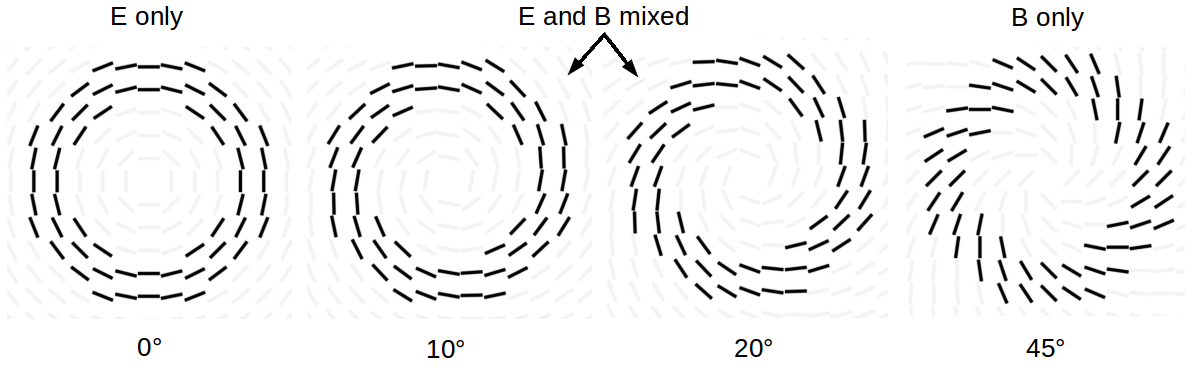
\includegraphics[width=\textwidth]{figures/ebmixing.png}
\caption{Visualization of a coherent polarization angle rotation and its effect on the E and B mode mixing.
}\label{fig:ebmixing}
\end{figure}

Sources of polarization angle systematics are varied and can be introduced
several places in the instrument. A few examples include 1) a rotating
elliptical beam, say in the case of a design incorporating bore-sight
rotations, causing T to P leakage (see ellipticity section); 2) off-axis
refractive optics influencing the propagation of the polarization vectors
according to their Fresnel coefficients, leading to an instrumental
polarization angle rotation; and 3) an apparent polarization angle rotation
from the detector time constants in the presence of a HWP (see time constant
section). Here we focus on 2), namely instrumental polarization errors and
detector polarization angle rotations.


A global polarization rotation is degenerate with a CPR angle and affects the
power spectra as described in \cite{Pagano2009, Keating2013}. 
The effect of a coherent polarization angle roation is to correlate the spectra by an angle $\theta$ such that the new $C'_{\ell}$ coefficients result in

\begin{equation}
\begin{split}
C_{\ell}^{\prime TE} &= C_{\ell}^{TE} cos(2\theta) - C_{\ell}^{TB} sin(2\theta)\\
C_{\ell}^{\prime TB} &= C_{\ell}^{TE} sin(2\theta) + C_{\ell}^{TB} cos(2\theta)\\
C_{\ell}^{\prime EE} &= C_{\ell}^{EE} cos^{2}(2\theta) + C_{\ell}^{BB} sin^{2}(2\theta) - C_{\ell}^{EB}sin(4\theta)\\
C_{\ell}^{\prime BB} &= C_{\ell}^{BB} cos^{2}(2\theta) + C_{\ell}^{EE} sin^{2}(2\theta) + C_{\ell}^{EB}sin(4\theta)\\
C_{\ell}^{\prime EB} &= \frac{1}{2} (C_{\ell}^{EE} - C_{\ell}^{BB}) sin(4\theta) + C_{\ell}^{EB}(cos^{2}(2\theta) - sin^{2}(2\theta))\\
\end{split}
\end{equation}

The standard cosmological model predicts that TB and EB identically vanish.
This prediction can be used to calibrate CMB polarimeters through a
self-calibration method \cite{keating13,kaufman14a}, at the expense of losing
detection capability on genuine physical quantities. This method is
particularly effective for high resolution and/or high sky coverage
experiments. However, the initial assumption is not true in the presence of
phenomena that produce non-vanishing TB and EB. In these cases self-calibration
loses accuracy and introduces biases on cosmological parameters
\cite{abitbol16}. 
Besides, this method destroys the possibility to measure or to place limits on
phenomena that generate TB and EB spectra, like Cosmic Birefringence, Faraday
Rotation and chiral gravity models \cite{kaufman14b,gerbino16}.


\paragraph{Plan to model and/or measure:}

Analytic description of instrumental rotation is challenging, necessitating the
use of optical modeling and experimental techniques for calibration of final
detector angles (absolute and relative) and systematic rotations from the
optics. It is critical to both model and measure the detector polarization angles.
Calibration should be performed before deployment and during observations. 

Modeling of the polarization rotation angle appears feasible and has been used
on ACTPol using Code V \cite{2016arXiv160701825K}. Polarization rotation can be
modeled in CODE V using a polarization sensitive ray trace. An input
polarization is defined and propagated through the optical chain to the
detector focal plane. The pupil averaged Stokes vector is then used to
calculate the polarization angle at the focal plane. This process is repeated
for 25 different fields on the sky and the results are fit to a 2D quadratic.
This fit is then used to estimate the rotation for each detector on the focal
plane. An example of the modeled rotation for the first Advanced ACT array is
shown in Figure \ref{fig:advact_pa4_pol_rotation}. A similar analysis can be
done in Zemax, though is known to not be accurate for fast optical systems.

\begin{figure}[h!]
\begin{center}
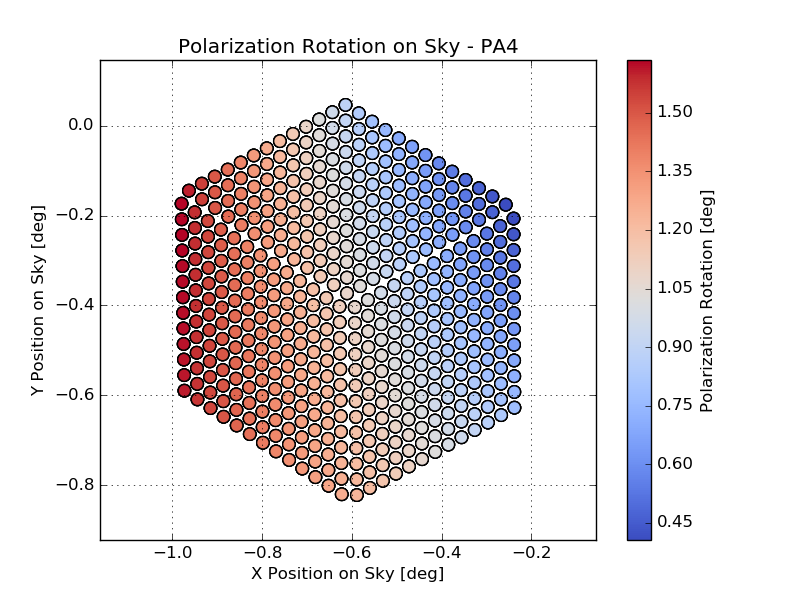
\includegraphics[width=0.60\linewidth]{advact_pa4_polarization_rotation_150ghz_2017.png}
\caption{Modeled instrumental polarization rotation for the high frequency (HF)
Advanced ACT array. Each circle represents a single feedhorn at the focal
plane. The color represents the amount of rotation as modeled by CODE V.}
\label{fig:advact_pa4_pol_rotation}
\end{center}
\end{figure}

This should be checked with physical optics calculations and measurements, but
can be performed on a proposed telescope design which includes both reflectors
and lenses.

Microwave detectors must be cooled down from 300 K to 100 mK, so differential
contractions of the materials in the cryostat limit the accuracy of their
aligment. It is also critical to refer the detector orientation with respect
to the telescope and the receiver mount once the cryostat is closed. As a
result, direct polarization angle calibration is not possible with an accuracy
better than 1$^{\circ}$.

We plan to use polarization calibrators in-lab while testing full optics tubes
before deployment, in situ in the field with polarization calibrators, either
through a ground-based calibrator, or utilizing a flying artificial source, and
observations polarized astrophysical sources. However, natural sky sources
traditionlly used to calibrate the absolute polarization angle suffer from
frequency dependence and time variability. The best option are Tau-A and Cen-A,
but they allow an accuracy for the polarization orientation between 1$^{\circ}$
and 0.5$^{\circ}$ \cite{planck16i,polarbear14,weiland11}. 

Placing a well known polarization calibrator in the far field of the telescopes
is the optimal approach, though quite challenging. Proposed ideas include
operating precisely characterized, linearly polarized microwave sources using a
drone, a balloon, or a CubeSat \cite{nati2017, Johnson2015}. These artificial
calibrators will match the sensitive frequency bands of the polarimeters and
will be observed at high elevation angles, far from Earth signal contamination.

The source is coupled to an attitute control system making use of star cameras
and other attitude sensors. The caibrator will utilize two celestial
coordinates (from the accurate star camera pointing direction) to determine the
third angle defining the rotation of the polarization plane along the
detectors' line of sight. The telescopes' detector orientation is then measured
by observing the calibration source signal. 

\textbf{Say something about the PB calibrator that Grant has been working on}.


Alternative calibrators require placement in the near field and include
sparse/dense wire grid polarizers or dielectric sheets \cite{Takahashi2010,
2016arXiv160701825K}.  However, any strategy based on optical elements placed
between the mirrors and the polarimeter does not allow to measure the polarized
beam systematics induced by the warm optics. 

\textbf{Note that it would be easier to measure in-lab if we only have the
optics tubes and what options we have for that. See the calibration hardware
spreadsheet linked on the CSS telecon page.}

The absolute calibration of the polarization angle is critical for the
detection of inflationary gravitational waves, the constraining power on the
neutrino sector through measurements of gravitational lensing of the CMB, the
possibility of detecting Cosmic Birefringence (CB), and the ability to measure
primordial magnetic fields, and thus has an SRF of 5.

\paragraph{Uncertainty/Range:}
%This section should include the uncertainty of
%known parameters and/or the expected range of parameters for consideration

Angle offsets $\sim 1^{\circ}$ produce spurious B-mode signal at the same level
as primodial B-modes for a tensor to scalar ratio of $r \sim 0.005$ as well as
nonzero $EB$ and $TB$ cross-correlations \cite{doi:10.1142/S0218271816400125}.
Currently employed calibration methods provide calibration to at
best $0.5^{\circ}$ \cite{2016MNRAS.455.1981K}.
Calibration to better than $0.05^{\circ}$ would allow for constraints on CB of
order one degree to greater than $15\sigma$ \cite{2016MNRAS.455.1981K}.

A miscalibration of 0.5$^{\circ}$ in the polarization orientation translates
into a spurious B-mode signal corresponding to a tensor-to-scalar ratio of $r
\simeq 0.01$ \cite{abitbol16}, affecting the SO sensitivity range.  Depending
on the targeted value for r, we need to calibrate the polarization angle with
arcmin or even sub-arcmin accuracy. 
A simulated result is shown in Fig. \ref{plot_r:fig} \cite{nati2017}, for an
ACT-like and a CMB-S3 experiment. Assuming  the red curve represents a false
bias signal introduced by a miscalibration of 1$^{\circ}$ (i.e., the current
accuracy) in the orientation of the detectors.  The bias starts to emerge above
the statistical uncertainty for ACTPol sensitivity (the image on the left). For
CMB-S3 (the image on the right), the new generation of ground experiments, the
bias is well above the sensitivity and it dramatically affects the measurement
of r. If the same experiment benefits from a calibration with accuracy between
0.01$^{\circ}$ and 0.001$^{\circ}$, the bias can be recovered as represented by
the blue region.
 
\begin{figure}[ht]
\begin{center}
\includegraphics[width=\textwidth]{figures/act_s3_r} 
\end{center}
\caption{Assuming no gravitational waves, the red curve in these simulations
represents a false detection of $r$ caused by the polarization angle
miscalibration of 1$^{\circ}$. With a calibration accuracy between
0.01$^{\circ}$ and 0.001$^{\circ}$ represented by the blue region, POLOCALC
\cite{nati2017} recovers the fiducial value of r=0 (the black dashed curve).
The uncertainty on the value of $r$ will be then limited by the sensitivity of
the experiment. The false bias already starts to emerge above the statistical
uncertainty for the ACTPol sensitivity, while for CMB-S3 it dramatically
affects the measurement of the tensor-to- scalar ratio. For CMB-4 the gap is
going to increment.}
\label{plot_r:fig}
\end{figure}

\paragraph{Parameterization:}
This effect can be parameterized by the polarization angle uncertainty, which
can be used to estimate the polarization power spectra leakages as in
\cite{nati2017}. This can be used to estimate the impact on our
science goals.

cience goals.

\subsection{Inhomogeneous AR Coating}

\paragraph{Description:}
If a telescope has any transmissive opitcal elements, those elements will need to have an effective antireflective (AR) coating.  Some systematics are particular to the AR technology used, but there are some general systematics.  Inhomogeneities can occur with most technologies, such as by a variation in the thickness of a layer across the element.  This will cause a decrease in the AR performance at the location of the inhomogeneity.  If the element is in a position in the beam such that all the detectors effectively see the entire element, this will be averaged over the entire element, and the systematic will be the same across the whole focal plane.  If the element is in a position such that each detector sees only a small part of the element, there will be a focal plane positional dependence on the transmission.  If there are several such elements in the optical path for each detector, the effect will hopefully average out over the focal plane.

\paragraph{Plan to model and/or measure:}
The AR coating performance of each element can be measured with a reflectometer. Measurements of specific technologies can give the tolerances of each technology. Using reflectometery, we can measure reflection vs. frequency data for these designs, understand the thickness and index tolerances of any proposed AR technology, and determine an rms for each layer of AR coating. Using the tolerances, rms values, and a transfer matrix model can give predictions on how much this will affect the overall AR coating performance. Given the reasonably tight tolerances of current technologies, this will not be a major problem and thus has a SRF of 2.

\paragraph{Uncertainty/Range:}
Most technologies can get to a paricular thickness consistency across the surface. This may be from $\pm$ 5 to 25 $\mu$m depending on the technology. Overall, this is a relatively small amount at most frequencies though at the upper end of ground-based range, it may start to present a problem. If the AR performance is tightly tuned across the band (to about 0.5\% or less across the band), then any deviation will cause the the performance to degrade to $\sim 1$\%. If the performance is closer to $\sim 1$\% or the coating has a very broad bandwidth, then this effect will shift the performace bands around by a few percent.  

\paragraph{Parameterization:}
The transfer matrix formalism with the measured tolerances and rms can give the total impact on the AR coating performance.

\subsection{Polarization Wobble : Sinuous Antenna}

A sinuous antenna is part of a class of planar antenna geometries called log-periodic antennas due to a log-periodic winding of the antenna arms. The benefit of log periodic antennas is the fact that their properties such as impedance, and beam properties stay consistent over a wide bandwidth and repeat every $ln(\tau)$ where $\tau$ is the characteristic length scale over which the antenna arm pattern repeats. The maximum and minimum bandwidth of these antennas are in theory just set by their inner and outer radii. One characteristic of log periodic antennas that is problematic for polarization measurements of the CMB is polarization wobble. This is a rotation of the polarization axis that oscillates between a maximum and minimum value every $\ln(\tau)$. Within the class of log-periodic antennas the sinuous antenna has the lowest amount of polarization wobble and the amount of antenna wobble is set by $\tau$: lower $\tau$ corresponds to smaller max to min deviation in polarization axis. Detailed studies of the PB2 sinuous antennas can be found in \cite{Obrient2008},\cite{Edwards2012}.


Polarization wobble is primarily a problem because is creates cross polarization or Q to U leakage, which translates into E to B leakage. The wobble can additionally induce temperature to B-mode leakage from the ellipticity angle not alligning with the orthogonal directions of the polarization axis. Systematics from PB2 antennas as well as detectors and lenslets can be found in some details in \cite{TokiThesis}.

\paragraph{Plan to model and/or measure:}
Minimizing $\tau$ minimizes cross polarization but smaller $\tau$ also sets the required linewidths of your traces. For POLARBEAR a $\tau$ of 1.3 was chosen to minimize $\tau$ but still allow for fabrication constraints on trace widths. To further null the effect of cross polarization from polarization wobble a 4 pixel differencing scheme has been proposed \cite{TokiThesis},\cite{TokiMemo1},\cite{TokiMemo2}, which will return Q and U values independent of the polarization wobble angle. This procedure requires two sets of two pixels each (A and B as shown in Fig.~1) with each set having one antenna with one linear polarization oriented at 0 degrees and the second pixel rotated by 45 degrees. The polarization wobble angle is denoted as $\phi(\nu)$, the angle of incident light is $\theta(\nu)$, the detectors efficiency is $\eta(\nu)$, and the electric field amplitude is $E(\nu)$. This setup is depicted in Figure~1. The steps to extract Q and U values for the 4 pixels with the dependence on $\phi(\nu)$ removed is described below. The relative power on the the 90 and 45 pixels of the A and B sets is given by
\begin{figure}
\centering
\includegraphics[width=2.5in]{figures/4pixelremovewobble.png}
\caption{Illustration of 4 pixels with polarization wobble. Each set A and B have both a 0 \& 90 degree orientation antenna and a 45 \& -45 degree orientation pixel. $\theta$ is the polarization angle of incoming light, and $\phi$ is the polarization wobble angle.}
\label{4pixelwobbleremoval}
\end{figure}
\begin{equation}
\begin{split}
&P_{A0} = \int \eta(\nu)[E(\nu)cos(\theta(\nu)-\phi(\nu))]^2 d\nu \\
&P_{A90} = \int \eta(\nu)[E(\nu)sin(\theta(\nu)-\phi(\nu))]^2 d\nu \\
&P_{A45} = \int \eta(\nu)[E(\nu)cos(\frac{\pi}{4}-\theta(\nu)+\phi(\nu))]^2 d\nu \\
&P_{A-45} = \int \eta(\nu)[E(\nu)sin(\frac{\pi}{4}-\theta(\nu)+\phi(\nu))]^2 d\nu \\
&P_{B0} = \int \eta(\nu)[E(\nu)cos(\theta(\nu)+\phi(\nu))]^2 d\nu \\
&P_{B90} = \int \eta(\nu)[E(\nu)sin(\theta(\nu)+\phi(\nu))]^2 d\nu \\
&P_{B45} = \int \eta(\nu)[E(\nu)cos(\frac{\pi}{4}-\theta(\nu)-\phi(\nu))]^2 d\nu \\
&P_{B-45} = \int \eta(\nu)[E(\nu)sin(\frac{\pi}{4}-\theta(\nu)-\phi(\nu))]^2 d\nu .
\end{split}
\end{equation}
We then assume that $\theta$ is constant across our spectral band and difference opposite orientation detectors to extract Q and U:
\begin{equation}
\begin{split}
&Q_A= P_{A0}-P_{A90}=\int \eta(\nu)E^2(\nu)cos[2(\theta-\phi(\nu))]d\nu \\
&Q_B = P_{B0}-P_{B90}=\int \eta(\nu)E^2(\nu)cos[2(\theta+\phi(\nu))] d\nu \\
&U_A = P_{A45}-P_{A-45}\int \eta(\nu)E^2(\nu)sin[2(\theta-\phi(\nu))] d\nu \\
&U_B =  P_{B45}-P_{B-45}\int \eta(\nu)E^2(\nu)sin[2(\theta+\phi(\nu))] d\nu \\
\end{split}
\end{equation}
Using the trig angle sum formula, we can expand this to
\begin{equation}
\begin{split}
&Q_A= \int \eta(\nu)E^2(\nu)[cos(2(\theta)cos(2\phi(\nu))+sin(2(\theta)sin(2\phi(\nu))]d\nu \\
&Q_B = \int \eta(\nu)E^2(\nu)[cos(2(\theta)cos(2\phi(\nu))-sin(2(\theta)sin(2\phi(\nu))]d\nu \\
&U_A = \int \eta(\nu)E^2(\nu)[sin(2(\theta)cos(2\phi(\nu))-cos(2(\theta)sin(2\phi(\nu))]d\nu \\
&U_B =  \int \eta(\nu)E^2(\nu)[sin(2(\theta)cos(2\phi(\nu))+cos(2(\theta)sin(2\phi(\nu))]d\nu . \\
\end{split}
\end{equation}
Taking linear combinations of the above Q's and U's we can define new Q's and U's as
\begin{equation}
\begin{split}
&Q_1=\frac{Q_A+Q_B}{2}= cos(2\theta)\int \eta(\nu)E^2(\nu)cos(2\phi(\nu))d\nu \\
&Q_2 = \frac{U_B-Q_A}{2}= cos(2\theta)\int \eta(\nu)E^2(\nu)sin(2\phi(\nu))d\nu \\
&U_1 = \frac{Q_A-Q_B}{2}= sin(2\theta)\int \eta(\nu)E^2(\nu)sin(2\phi(\nu))d\nu \\
&U_2 =  frac{U_A+U_B}{2}= sin(2\theta)\int \eta(\nu)E^2(\nu)cos(2\phi(\nu))d\nu. \\
\end{split}
\end{equation}
You can then extract $\theta$ as
\begin{equation}
\theta=\frac{1}{2}tan^{-1}\frac{U_{1,2}}{Q_{2,1}}.
\end{equation}
The E-field amplitude can also be determined form this scheme as:
\begin{equation}
E^2=\frac{P_{A0}+P_{A90}}{\int\eta(\nu)d\nu}=\frac{P_{A45}+P_{A-45}}{\int\eta(\nu)d\nu}=\frac{P_{B0}+P_{B90}}{\int\eta(\nu)d\nu}=\frac{P_{B45}+P_{B-45}}{\int\eta(\nu)d\nu}
\end{equation}
Where $\eta(\nu)$ is measured using an FTS. 

The polarization wobble is a large effect that causes significant leakage into the B-mode spectrum, but it is well-understood. It thus needs to be modeled and mitigated, making its SRF a 4.

\paragraph{Uncertainty/Range:}
This analysis assumes that all channels have the same response $\eta(\nu)$, but there is some variation across detectors, so uniformity across the array can limit the effectiveness of this method. This method also requires accurate FTS measurements of the spectral response. It also assumes that the beams are perfectly symmetric, so further uncertainty can be introduced from ellipitical beams. For a trypical sinuous detector, the ellipticity is small with a level of $<2$\% and varies with frequency. \textbf{What are additional sources of uncertainty?}

\textbf{How much suppression of the E to B leakage does this method provide? How much suppression of the T to B leakage does it provide?}

\paragraph{Parameterization:}
The leakage from the polarization wobble can be parameterized as the contaminated Q and U maps to estimate the power spectra leakages. Using the four pixel subtraction method in map space can determine how well these leakages can be mitigated.

\textbf{Make sure these commented out references are in the systematics dictionary references}
%\subsubsection{References}
%\begin{itemize}
%\item O'Brient, B. \textit{et.al.}, "Sinuous-Antenna coupled TES bolometers for Cosmic Microwave Background
%Polarimetry," LTD13 Proceedings (2009).
%\item Edwards, J.M. \textit{et.al.}, "Dual-Polarized Sinuous Antennas on Extended
%Hemispherical Silicon Lenses," IEEE Trans Antennas and Propagation, Vol 60, No 9 (2012).
%\item Suzuki, A. "Lenslet Coupled Sinuous Antenna Systematic Study", Berkeley Memo (2015). - Ask for this, its not published.
%\item Suzuki, A. "Sinuous Antenna Wobble Cancellation", Berkeley Memo (2012). - Ask for this, its not published.
%\item O'Brient, B. \textit{et.al.}, "Sinuous Antennas for Cosmic Microwave Background
%Polarimetry," SPIE, Vol 7020 70201H-1 (2008).
%\item Suzuki, A. "Multichroic Bolometric Detector Architecture for Cosmic Microwave Background Polarimetry Experiments," Berkeley Dissertation (2013).
%\end{itemize} 

\subsection{Misalignment of Lenslet/Horn Array}

\paragraph{Description:}
With the lenslet coupled antenna technology, there is a possibility that the lenslets will not be aligned with an antennae. This can occur with individual pixels or the entire wafer. In the case of individual pixels, this offset would be in random directions across the wafer and thus average out across the array. In the case of entire of wafer, misalignment can be caused cause by how well the wafer and lenslet array are clamped together and thermal contraction between the wafer holder and the wafer. An entire wafer offset would create a systematic pointing error.

\paragraph{Plan to model and/or measure:}
We can create a model in HFSS to simulate the effect on beam parameters from a systematic misalignment between a lenslet and an antenna. We can then use Zemax/Grasp to propagate the beam to the sky and estimate how much this effect contributes to the pointing error. If the location of the wafer and its orientation relative to a beam mapper, the pointing offset could be measured in lab, but this could be difficult in practice. In the field, the pointing offset can be characterized with point source observations (either on a tower/drone in the farfield or celestial) as described in the previous sections as part of the full pointing model.

PB2 models of this effect show a linear relationship between the pointing error and the offset between the lenslet and antenna (see Figure~\ref{poitingoffsetFromWaferslipped}). The direction of thepointing offset is in the same direction as the wafer slip. 
  
\begin{figure}
\centering
\includegraphics[width=3.25in]{figures/pointingOffset_waferslipped.png}
\caption{Pointing error versus an offset between a sinuous antenna and a lenslet for PB2. The pointing offset roughly linear with the offset between the two.}
\label{poitingoffsetFromWaferslipped}
\end{figure}


We can model this effect well, but need to model it, making its SRF a 3.

\paragraph{Uncertainty/Range:}
We can minimize the uncertainty from this effect by understanding the effects that can cause a wafer to slip like thermal contraction from the wafer holder and wafer or outside vibrations and setting contraints on wafer slippage. The range of the uncertainty also varies with the size of lenslets and antenna. In the PB2 case, we set the tolerance level at 20 $\mu m$. \textbf{Do we have some tolerance numbers for SO?}

\paragraph{Parameterization:}
We parameterize this effect as a pointing offset.

\input{tex/feedhorn_crosspol.tex}
\subsection{Polarization Leakage from Detector Array}

\paragraph{Description:}

Beam asymmetries from the optical coupling to the array can cause leakage from temperature to polarization and E-modes to B-modes. The beams need to be modeled and measured so that they can be correctly incorporated into the analysis to minimize these effects.

\paragraph{Plan to model and/or measure:}
The simplest way to model this effect is by assuming a pair-differenced detector. In the case that a HWP is used, this effect is mitigated because there is no pair differencing. To estimate this effect with a HWP, one would have to propagate the analysis through a demodulated timestream, but this method is still useful in this case because it can give an upper limit on the effect. In the non-HWP case, the polarization angle of the detector can be used instead of pair-differencing to determine the polarized signal.

The polarization leakages in the power spectra are estimated using the simulated co- and cross-polar beams from HFSS. Assuming a pair-differenced detector, the electric fields on the sky $E_x$ and $E_y$ are coupled to the electric field in the detectors $E_a$ and $E_b$ by
\begin{equation}\label{eqn:beams}
  \begin{bmatrix}
  E_a\\
  E_b
  \end{bmatrix}
  =
  \begin{bmatrix}
  \beta_{ax} & \beta_{ay}\\
  \beta_{bx} & \beta_{by}
  \end{bmatrix}
  \begin{bmatrix}
  E_x\\
  E_y
  \end{bmatrix}
  \,\,\, ,
\end{equation}
where $a$ and $x$ as well as $b$ and $y$ are aligned along the boresight. Here $\beta_{ax}$ and $\beta_{by}$ are the co-polar beams, and $\beta_{ay}$ and $\beta_{bx}$ are the cross-polar beams. The default setting in HFSS is to source the calculation through the wave port in the $x$ direction, which gives $\beta_{ax}$ and $\beta_{ay}$. To model $\beta_{bx}$ and $\beta_{by}$, the source must be changed to the wave port in the $y$ direction. The complex beams are then given by the sum of their real and imaginary parts as
\begin{align}
\beta_{nx} & =  \mathrm{Re}(rEL3X)+i\, \mathrm{Im}(rEL3X) \nonumber \\
\beta_{ny} & =  \mathrm{Re}(rEL3Y)+i\, \mathrm{Im}(rEL3Y)\,\,\,\,\,,
\end{align}
where $n$ is either $a$ or $b$. The co- and cross-polar beams from HFSS are then masked such that they go to zero outside of the Lyot stop, and a 2D FFT is performed to estimate the far field beams~\cite{Simon_Thesis_2016}.

For an ideal bolometer differencing pair at the output of the of the horn, the measured polarized signal $P$ would be
\begin{equation}\label{eqn:p1}
P=E_a-E_b \,\,\,\,.
\end{equation}
The Stokes parameters using the decreasing phase convention are given by
\begin{align}\label{eqn:Stokes}
I & =  |E_{x}|^2+ |E_{y}|^2  \nonumber \\
Q & =   |E_{x}|^2- |E_{y}|^2  \nonumber \\
U & =  2\,\mathrm{Re}(E_{x} E_{y}^{*}) \nonumber \\
V & =  2\,\mathrm{Im}(E_{x} E_{y}^{*})\,\,\,\,\,.
\end{align}
Here $I$ is the intensity, $Q$ and $U$ describe the linear polarization, and $V$ describes the circular polarization. Substituting Equation~\ref{eqn:beams} into Equation~\ref{eqn:p1} and using the definition of the Stokes parameters  as in Equation~\ref{eqn:Stokes} gives
\begin{equation}
P=\sigma I + \delta Q + \epsilon U+ \gamma V\,\,\,\, ,
\end{equation}
where the coefficients are the beam couplings from $I$, $Q$, $U$, and $V$ into $P$. For an ideal detector, $\delta=1$ and $\sigma=\epsilon=\gamma=0$. The beam couplings are then given by
\begin{align}\label{eqn:leakage beams}
\sigma & =  \frac{1}{2} (\beta_{ax}^2 + \beta_{ay}^2 - \beta_{bx}^2 - \beta_{by}^2) \\
\delta & =   \frac{1}{2} (\beta_{ax}^2 - \beta_{ay}^2 - \beta_{bx}^2 + \beta_{by}^2) \\
\epsilon & =  \mathrm{Re}(\beta_{ax}^{*} \beta_{ay} - \beta_{bx}\beta_{by}^{*} )  \\
\gamma & =  -\mathrm{Im}(\beta_{ax} \beta_{ay}^{*} + \beta_{bx}^{*}\beta_{by} )\,\,\,\,\,.
\end{align}
The beams are then normalized by the maximum of $\delta$ and averaged across each observation band. A more sophisticated analysis could weight the frequency average by the total bandpass. As the distance from the center of the array increases, the ellipticity of the Lyot stop as viewed from the pixel increases, which results in higher leakage. The central pixel thus gives the lowest temperature to polarization leakage. While edge pixels exhibit higher leakage, the average leakage beam of pairs of pixels equidistant from the array center on opposite sides of the array approximates the behavior of the central pixel. Therefore, the behavior of the central pixel can provide an estimate for the systematics of the array~\cite{Simon_Thesis_2016}.

We estimate the leakage in the power spectra from these band-averaged beams with two methods: a map-based systematics pipeline and a window function method. The map-based method gives a full estimation of this effect using the leakage beams and simulated maps and realistic noise estimates. This method is useful for determining how much of the temperature to polarization leakage goes into E-modes versus B-modes. With the window function method, the leakage is estimated using the calculated window functions of the signal and leakage beams. This simplified model is quick to model, but only gives total polarization leakage versus how much of the leakage goes into E-modes versus B-modes. However, it is still good as a check on the worst-case scenario. For feedhorns, the main source of the leakage is from ellipticity. Based on symmetry arguments presented in Shimon et al., 2008~\cite{Shimon_2008}, the temperature to polarization leakage goes largely into E-modes, and the E-mode to B-mode leakage is negligible. Simulations from the map-based pipeline also show that this is the case. Because of the wobble effect in a sinuous antenna coupled to a lenslet, the temperature to polarization leakage has a large contribution to the B-modes, and the E-mode to B-mode leakage is large.

In the window function method, for each beam, the magnitude squared of the FFT of the averaged far field beams is calculated and normalized by the maximum of the transformed $\delta$ beam. Next the 2D functions are binned radially to make a 1D window function.  

%To account for the rest of the telescope optics, one can normalize the multipole axis by comparing the $\delta$ window function to a window function of a Gaussian beam with full width at half maximum (FWHM) equal to that expected at a given center frequency of each observation band from optics modeling. 

The measured spectra are then estimated by multiplying simulations of the EE and BB polarization spectra by the $\delta$ window function, the temperature to polarization leakage spectrum is determined by multiplying the simulated TT spectrum by the $\sigma$ window function, and the EE to BB leakage is determined by multiplying the simulated EE spectrum by the $\epsilon$ window function. 

In general, as pixel size increases, the feedhorn optimization has more aperture to work with, so the systematics level decreases in both bands. The decrease in the lower band is usually smaller because the waveguide cutoff of the horn can cause beam distortion. This effect can be modeled more precisely with the full bandpass weighted beam average. Feedhorns are also tunable in their design based on the penalty function used for optimization, so if the systematics levels are ever too high for a given design, the horn optimization can sacrifice beam coupling efficiency for better symmetry and vice versa. For the sinuous and lenslet case, as pixel size increases, there is no overall decrease in the level of systematics. Instead, as the pixel size increases, the level of leakage in the high band increases, while the level of the leakage decreases in the low band and vice versa.

Cross-linking in the maps can help identify and quantify this leakage. Accounting for beam asymmetries in the analysis can mitigate the leakage by an order of magnitude or more. The level of this mitigation is dependent on how well the telescope beams are characterized by planets, point sources, and/or calibration sources. Prior to deployment, we can use beam measurements from a warm vector network analyzer and cold beams in lab to characterize the detector array beams isolated from the rest of the optics. Additional mitigation is needed both in the design of the arrays and the analysis for the lenslet and sinuous detector arrays since mitigating the wobble effects necessitates the use of the four-pixel subtraction scheme. In the SAC, the use of HWPs is expected to mitigate this effect by a factor greater than 10.


\paragraph{Uncertainty/Range:}
Ideally, any leakage into the polarized spectra should be lower than the B-mode signal by several orders of magnitude. The EE to BB leakage is negligible for the feedhorn in both the LAT and SAC cases. For the lenslet and sinuous detector, the EE to BB leakage is at the level of the B-modes without any mitigation for both the LAT and SAC cases. Window-function simulations for the LAT, show that the total polarization leakage is several orders of magnitude below the B-mode signal for both the feedhorn and lenslet architectures. For the SAC, which has a larger stop, the level of the temperature to poalrization leakage is comparable to the level of the B-modes so the full map-based pipeline must be employed. Using this method, it can be determined that the feedhorn and lenslet architectures both have acceptable levels of leakage (when only the wobble mitigation for the lenslet is included). However, it is also imporatant to note that the SAC will have a HWP, which will strongly mitigate this effect.
%put some images for 5.3 mm case on SO.

%An example of this for the AdvACT 150/230~GHz feedhorns is shown in Figures~\ref{fig:HF_measured_spectra}, \ref{fig:HF_TP_leakage}, and \ref{fig:HF_EB_leakage}~\cite{Simon_Thesis_2016}.

\begin{figure}[h!]
\centering
\includegraphics[width=\textwidth]{figures/HF_measured_spectra.pdf}
\caption{Simulated measurements of the EE and BB polarization spectra using the 150/230~GHz AdvACT feedhorn candidates are shown above for the 150~GHz band (left) and the 230~GHz band (right)~\cite{Simon_Thesis_2016}.}
\label{fig:HF_measured_spectra}
\end{figure}

\begin{figure}[h!]
\centering
\includegraphics[width=\textwidth]{figures/HF_TP_leakage.pdf}
\caption{The temperature to polarization leakage of the AdvACT 150/230~GHz spline-profiled (red), conical (cyan), and corrugated (magenta) feedhorns are plotted with the B-mode signal for $r=0$ (green) and $r=0.01$ (blue) for the 150~GHz band (left) and the 230~GHz band (right)~\cite{Simon_Thesis_2016}.}
\label{fig:HF_TP_leakage}
\end{figure}

\begin{figure}[h!]
\centering
\includegraphics[width=\textwidth]{figures/HF_EB_leakage.pdf}
\caption{The EE to BB leakages of the AdvACT 150/230~GHz feedhorn candidates are shown above for the 150~GHz band (left) and the 230~GHz band (right). In all cases, this leakage is negligibly low~\cite{Simon_Thesis_2016}.}
\label{fig:HF_EB_leakage}
\end{figure}


\paragraph{Parameterization:}
This can be parameterized with the estimated leakage spectra from the pair-differenced model or with the feedhorn beams from HFSS should more detailed modeling be desired.





\section{Spectral Response Function}
\subsection{Bandpass Mismatch}

\paragraph{Description:}
Different detectors can have different bandpasses from effects like fabrication variations. 

%The total power received by a detector is the sum of each source of light coming from the sky integrated over the bandpass of the detector. Given that each component of the signal has a different spectrum, the calibration of the detector is component dependent. For each component $k$ and bolometer $b$, we can define a transmission coefficient
%\begin{equation}
%C_k^b = \frac{\int S_k(\nu) F(\nu)}{\int S_{CMB}(\nu) F(\nu)}.
%\end{equation}
%These correction factors to the gain should be applied whenever the signal has a different frequency dependance than the CMB. If not accounted for, this will result in a mis-calibration like effect for all of the foregrounds, producing temperature-to-polarization and polarization-to-polarization leakage.

Power spectra leakages also manifest when two detectors with non-identical spectra are pair-differenced to get a polarized signal. \textbf{expand on this a bit}

\paragraph{Plan to model and/or measure:}
The only way to mitigate this effect is with spectral measurements of the detector bandpasses using a Fourier Transform Spectrometer (FTS). For these measurements to be effective, we must have wide coverage across each array so that we can characterize any wafer variations and better understand idividual detector bandpasses. FTS measurements for each detector should be performed in the lab prior to deployment and in situ in the field.

\textbf{Discuss how the size of a mismatch can be modeled by changing the dielectric thickness in the filter to model fabrication variance. Describe how with this, we can model the maximal band offset, with that, we can tell how well we need to know the detector bandpasses. Discuss how this can then be used to set FTS calibration requirements and also for requirements on detector fab array uniformity.}
%Using external foregrounds maps as templates, the leakage maps can be computed and subtracted. However, this method is limited by our knowledge of the foregrounds, and the external available data. Simulations to estimate the level of leakage and set a constraint on the differential bandpasses should be performed.

This effect can cause polaization leakage and requires thorough instrumental calibration, making its SRF a 4. This effect is less worrying when pair-differencing is not used, as in the case of a HWP, which brings its SRF down to 3.

\paragraph{Uncertainty/Range:}
\textbf{How well do we need to know each detector bandpass for the spectral effect? for pair differencing? What requirements do these put on FTS calibration? Do we need R and D to reach these levels of calibration or are we already there? How much of an array do we need to understand? Do we need FTS measurements of every array?}

\paragraph{Parameterization:}
This effect can be parameterized as an uncertainty on the center frequency and bandwidth of the detectors, which can be used to estimate the limitations on the proposed science, particularly on how well we can constrain $r$.


\section{Polarization Modulators}
A Half Wave Plate (HWP) is an optical device that introduces a phase delay between the two orthogonal polarizations of the incoming signal. It can be made of birifringent crystals (e.g. Sapphire) or metamaterials. The HWP flips the polarization of incoming light along the fast axis of the crystal resulting in a polarization shift of $2\chi$, where $\chi$ is the incoming polarization angle of the light with respect to the fast axis. Thus, a HWP rotating with frequency $f$ mo\-du\-la\-tes the incoming polarization at $2f$, which is detected in the bolometer timestreams at $4f$. The demodulation process described below summarizes the formalism defined in Kusaka \& Essinger-Hileman et al., 2014~\cite{ABS_HWP}.

The detector timestream $d_{m}$ is composed of the unpolarized sky intensity $I$, the modulated polarization signal $P(\chi)$, white noise $N_{w}$, and spurious modulation signals $A(\chi)$ that depend on the HWP angle $\chi$ such that
\begin{equation}
d_{m}= I + P(\chi)+ N_{w} + A(\chi).
\end{equation}
The modulated polarization signal can be represented in terms of the Stokes $Q$ and $U$ parameters, eq.~(\ref{eqn:Stokes})), as
\begin{equation}
P(\chi)=\epsilon \mathrm{Re}\{(Q+iU) m(\chi)\},
\end{equation}
where the modulation is given by $m(\chi)=\exp[-4 i \chi]$ and $\epsilon$ is the polarization modulation efficiency factor, which is close to one. The spurious modulation signals $A(\chi)$ consist of components at every harmonic $n$ of the HWP rotation frequency and can be decomposed into cosine and sine components as
\begin{equation}\label{eqn:achi}
A(\chi)= \sum_{n} A_n(\chi)=\sum_{n}\Big[ (A^{nc}_{0} + \lambda^{nc} I) \cos(n\chi) + (A^{ns}_{0} + \lambda^{ns} I) \sin(n\chi)    \Big].
\end{equation}
Here the $A_{0}$ terms are stable and independent of the sky intensity and the $\lambda$ terms are small~\cite{ABS_HWP}.

The demodulated timestream is, then, extracted by applying a bandpass filter to $d_{m}$ to account for the slight variations in $f$, multiplying $d_{m}$ by $m^*(\chi)$, and applying a low-pass filter that passes $f\lesssim2$~Hz to eliminate higher order terms and all $A^{nc,s}$ and $\lambda^{nc,s}$ terms other than the $n=4$ components. From~\cite{ABS_HWP}, the final demodulated timestream $d_{\bar{d}}$ is then given by
\begin{equation}
d_{\bar{d}}=\frac{1}{2}\Big(\epsilon Q + A^{4c}_{0} + \lambda^{4c} I \Big) + N^{\mathrm{Re}}_{w} + \frac{i}{2}\Big(\epsilon U + A^{4s}_{0} + \lambda^{4s} I \Big) + iN^{\mathrm{Im}}_{w}.
\end{equation}

The optical action of a single layer birifringent material or achromatic metamaterial HWP can be described by the Mueller matrix:
\begin{equation}
M=\begin{bmatrix}
   t  &\rho  &0  &0\\
   \rho  &t  &0  &0\\
   0  &0  &c  &-s\\
   0  &0  &s  &c
\end{bmatrix}.
\label{eq:Mueller_Matrix}
\end{equation}

The $t$ term is proportional to the total unpolarized intensity transmitted by the HWP, the $\rho$ term to the differential transmission of the HWP. The $c$ and $s$ terms are responsible for the modulation of the polarized components, the $\rho$ term for the unpolarized ones. For an ideal HWP: $t=1$, $\rho=0$, $c=-1$, $s=0$. Deviations from these values are due, e.g., to the spectral behavior of the birifringent material/metamaterial (as we will deeply investigate in the next sections). The left panel of Fig.~\ref{fig:Mueller_elements} shows the Mueller matrix elements $M_{ij}$ for a single-layer HWP as a function of the frequency of the incoming radiation. 

\begin{figure}
\begin{center}
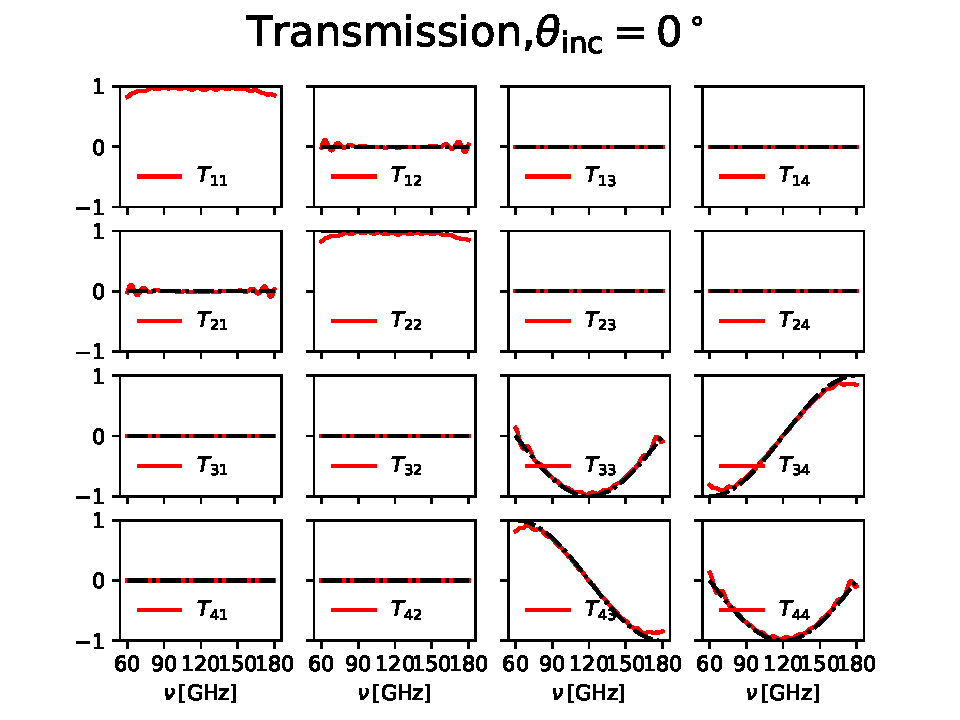
\includegraphics[0.5\linewidth]{plot/1layer_AHWP_120.pdf}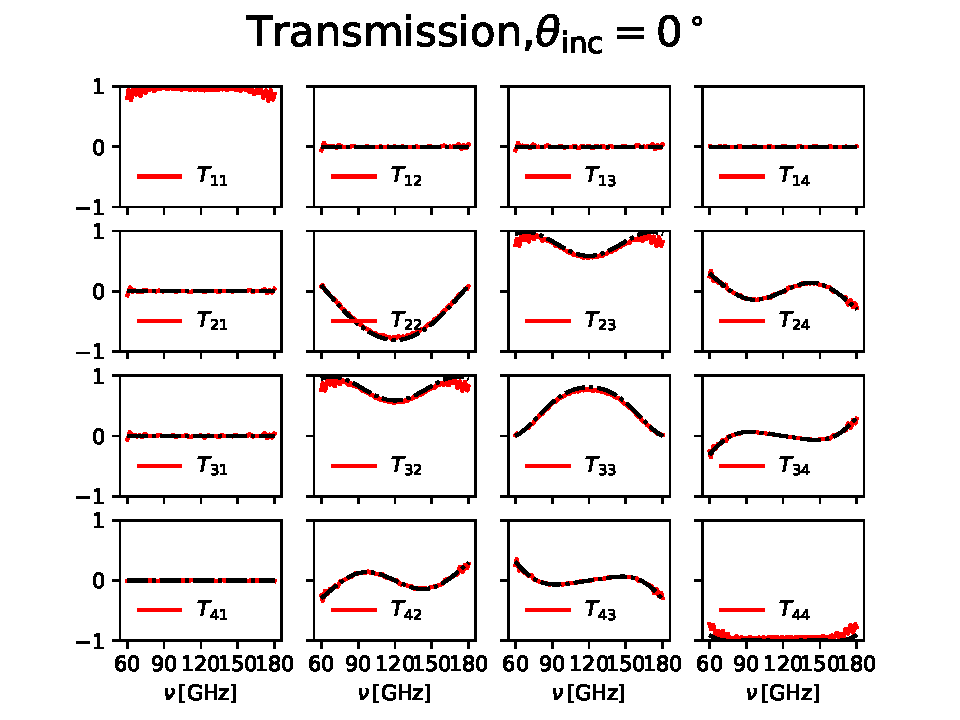
\includegraphics[0.5\linewidth]{plot/3layer_AHWP_120.pdf}
\end{center}
\caption{Mueller matrix elements $M_{ij}$ for a single-layer HWP (left panel) and a three-layer AHWP (right panel) as a function of the frequency of the incident radiation. Each layer is a made of Sapphire crystal and it is optimized for a central frequency of $120\,\mathrm{GHz}$. The AHWP is optimized to cover the broad-band range including the $90\,\mathrm{GHz}$ and $150\,\mathrm{GHz}$ frequency bands. The behaviour of $M_{ij}$ with the frequency for the single-layer HWP agrees with the description in eq.~(\ref{eq:Mueller_Matrix}). The behaviour of $M_{ij}$ for the AHWP is more complicated and agrees with the combination of three Mueller matrices as in eq.~(\ref{eq:Mueller_Matrix}) and rotated with respect to each other. Further details are provided in Sec.~\ref{subsec:modeff}. In both panels, the black dashed-dotted lines correspond to the elements of an ideal HWP.}\label{fig:Mueller_elements}
\end{figure}

For an achromatic HWP, made of stacks of birifringent material, the Mueller matrix presents further non-zero terms with respect to the ones in eq.\,(\ref{eq:Mueller_Matrix}), see Sec.\,\ref{subsec:modeff}. The right panel of Fig.~\ref{fig:Mueller_elements} shows the Mueller matrix elements $M_{ij}$ for a three-layer AHWP as a function of the frequency of the incoming radiation. The presence of additional non-zero elements with respect to the single-layer HWP is clearly visible. 

The HWP optical action creates a non zero $c$ and $s$ terms. Because this does not depend on the direction of the incoming radiation (upwards or downwards), the HWP Mueller matrix has the same shape, eq.\,(\ref{eq:Mueller_Matrix}), both in transmission and in reflection; the value of the corresponding Mueller matrix components changes according to the amplitudes of the electric field transmitted and reflected by the HWP.









% !TEX root =  ../syst_master.tex 

\subsection{Differential Optical Properties of a HWP}
\label{HWP Differential Optical Properties}

\paragraph{Description:}
Because the HWP is birefringent, the HWP has different transmission coefficients along the fast and slow axes of the crystal,
which produces differential absorption and emission coefficients along the two axes. Because of this, transmitted unpolarized light and emitted light both are partially polarized by the HWP. The polarization direction rotates with the HWP, so this signal couples to the detectors at 2$f$. While the science band is at $4f$, the $2f$ signal can leak into the $4f$ signal through... \textbf{fill this out a bit}.

\paragraph{Plan to model and/or measure:}
To model this effect, we require the HWP Mueller matrix and information about the optical filter chain. Knowing the temperatures, efficiencies, and emissivities of each component in the optical chain,
the unpolarized power can be propagated through each element to find the incident unpolarized power on the HWP.
If $P_n$ is the unpolarized power crossing the $n^\text{th}$ element, $\eta_n$ the efficiency, $\varepsilon_n$ the emissivity, and $B$ the spectral brightness, given the temperature $T_n$,
the propagation step is 
\begin{equation}
\label{unpolarized_propagation}
P_{n+1}(\nu) = \eta_n(\nu) P_n(\nu) + \varepsilon_n(\nu) A\Omega(\nu)\;  B(\nu, T_n) .
\end{equation}


The HWP Mueller matrix (Equation~\ref{eq:Mueller_Matrix} is calculated using the method described in \cite{Salatino16}, where all elements are dependent on frequency, incident angle and spatial position (x,y). The $\rho$ components represent the differential transmission of the HWP. While the polarized fraction of the transmitted and emitted light are equal and opposite, they do not cancel because the radiation sources are at different temperatures.
If we define $P_\text{HWP}$ to be the incident power on the HWP, the polarized power output is 
\begin{equation}
\label{eq:polarized_output}
P_\text{HWP + 1}(\nu) = \rho(\nu)(P_\text{HWP} - A\Omega(\nu)B(\nu, T_\text{HWP})),
\end{equation}
with $A_2 = \rho$. 

If we define $\eta_\text{det}$ to be the combined efficiency of all elements after the HWP,
the final 2$f$ signal produced by the HWP is 
\[
A^{(2)} = \int_{\nu_\text{low}}^{\nu_\text{high}} \eta(\nu) P_\text{HWP + 1}(\nu) d\nu.
\]

\textbf{How do we model how much leaks into $4f$ frmo $2f$?}

Since this effect can leak into the science band, it is important to model and thus has an SRF of 3.
\paragraph{Uncertainty/Range:}
For 145 GHz, this method gives values of $a_2 = .35\%$, and a value of 
$A^{(2)} = .0165 \text{pW} = 238 \text{mK}_\text{CMB}$. 
\textbf{We expect similar values for similar frequency values}.
\textbf{Describe how much of this leaks into $4f$ and contaminates our actual science signal.}

\paragraph{Parameterization:}
We require $T$ and $\rho$ from the HWP Mueller matrix\cite{Salatino16}, and an optical chain input file containing
absorption, temperature, and spill/scatter/reflection coefficients for each element. The Mueller matrix components can be theoretically estimated by transfer matrix model \cite{Essinger-Hileman13} or HFSS simulations. They can be experimentally measured with FTS measurements. We parameterize this with the $A_2$ component of the HWP template and a leakage coefficienct ($\epsilon_{2,4}$) between $2f$ and $4f$.


% !TEX root =  ../syst_master.tex 
\subsection{HWP $I \rightarrow P$ Leakage Originated from Differential Optical Properties of a HWP} 

\paragraph{Description:}
Though light polarized by the HWP primarily contributes to the 2$f$ component, a small amount of it can be modulated 
up to 4$f$.
This occurs when reflection induced polarization caused by irregularies in the AR coating is rotated by the HWP\cite{Essinger-Hileman2013, Essinger-Hileman2016, ABS_HWP}. 
Because it is reflected light being leaked into the 4$f$ signal, this can come from both upstream and downstream from the HWP.

\paragraph{Plan to model and/or measure:}
The leakage can be modelled with a transfer-matrix model of the HWP, and end-to-end pipeline simulations can be used to measure the total leaked polarization power.
To measure the leakage, one can measure 4$f$ as a function of sky I/PWV (Precipitable Water Vapour), or alternatively make maps of known unpolarised sources (like Jupiter) in the instrument Q/U frame
and measure the polarization. However both these method will characterize the overall $I \rightarrow P$ upstream of the HWP rather than just the HWP $I \rightarrow P$.
Any detector non-linearity will also Any detector non linear behavior will also contribute to this systematic effect (see Sec.\,\ref{det_nonlinearity}). 


\paragraph{Parameterization:}
The leakage coefficients are the elements $M_{12}$ and $M_{34}$ (or $\rho$ and $s$ of Sec.\,\ref{HWP Differential Optical Properties}) of the HWP mueller matrix M. These coefficients can be expanded into a beam Gauss-Hermite functions, 
see Equation 8 of \cite{Essinger-Hileman2016}. 

\paragraph{Uncertainty/Range:}
The effect is estimated to be small, in ABS, monopole leakage is 0.01\% and higher order leakage < 0.07\% \cite{Essinger-Hileman2016}.
Range comes from differential emissivity and transmission of the sapphire, reflection of radiation from the detectors to the HWP and back to detectors, 
misalignment of HWP axes. $I \rightarrow P$ leakage effect increases at non-normal incidence.

\subsection{Thermal Variation in HWP Temperature}

\paragraph{Description:}
In practice, the HWP has thermal gradients and fluctuations. A non-uniform HWP temperature and its temporal fluctuations create spatial and time dependent 0$f$, 1$f$, 2$f$, and 4$f$ signals that depend on the amplitude of the harmonic decomposition of the temperature profile of the HWP. 

\textbf{Add a few sentences about how estimating the HWP template wrong because it is spatially and temporally varying can translate into leakage.}

\paragraph{Plan to model and/or measure:}
To model this effect, we can use a thermal finite element analysis of a HWP thermalized with a suitable heat sink and with realistic time variable loading. \textbf{How can we estimate the next step (the impact on leakage from this)?}
To measure this, we can use cryogenic measurements of the thermal gradients, and on-sky measurements of polarization leakage will include this effect (as well as other instrumental sources)

This effect is expected to be subdominant, so the SRF is 3.


\paragraph{Uncertainty/Range:}
The uncertainties in these models will be limited by how realistic models of the time variation of the loading are. For a sapphire HWP, we expect the time variation effect to be small, as sapphire has a large thermal conductivity and large heat capacity, giving it both good thermalization properties and a large time constant.
 \textbf{Add more detail if we model this.}

\paragraph{Parameterization:}
We can parameterize this using the HWP thermal fluctuations: $\Delta_{HWP}(x,y,t)$ with $(x,y)$ the spatial coordinates of the HWP and $t$ the time and the effect on the HWP thermal fluctuation time constant: 

\begin{equation}
\tau_{T_{HWP}} = C(T_{HWP})/G(T_{HWP}, T_{BCK})
\end{equation}

where $C$ is the HWP heat capacity as a function of its temperatue $T_{HWP}$, and $G$ is the thermal link between the HWP at $T_{HWP}$ and the surrounding environment at $T_{BCK}$. 

Using this, we expect the HWP temperature to fluctuate, assuming a fluctuating background at frequency $\omega_{BCK}$, as

 \begin{equation} 
 T_{HWP} \propto \frac{e^{i \omega_{BCK} t}}{i \omega_{BCK} + 1/\tau_{T_{HWP}}}
 \end{equation}
 
 Because the time constant is large, we expect the thermal fluctuation to manifest at very low frequencies $\omega_{BCK}$. To estimate the scientific impact, we could parameterize this with spatially and temporally varying HWP template values.


\subsection{HWP Beam Systematics}


\paragraph{Description:}
Having a HWP skyward of every optical element mitigates a range of beam and polarization systematics. However, when the HWP is further down the optical chain as in the case of a cryogenic HWP, detailed modeling is necessary to determine what systematics it induces and mitigates.

\textbf{Do we have examples of what beam properties get worse?}

\paragraph{Plan to model and/or measure:}
Modeling would require the HWP optical properties and both ray tracing and physical optics for several cases, including non-planar positions and non-uniform AR coatings. The HWP would need to be included in full optics simulations of the optics chain. Commercially available software like CST can model diffraction effects, in a reasonable CPU time, for complicated, large structures, so a model could be developed for the HWPs and serve as input to the larger optical studies.

\textbf{Is there more info on how we can model/measure/calibrate/mitigate this effect? How do we account for mitigation and effects when it is included in the full optics configuration}

Beam maps with and without the HWP can also help determine the HWP's impact on the beams. Measurements, in principle, would be done with a long campaign of beam maps taken at a large set of HWP angle, and/or, in the case of a rapid modulator, very slow beam maps taken with several modulation cycles per beam scanned (differently from sky configuration where the telescope scan is faster). Both unpolarized and polarized beam maps would be necessary.

Optical effects of the HWP must be modeled as there is a large uncertainty in the size of the effect, so the SRF is 5.

\paragraph{Uncertainty/Range:}
\textbf{Do we have any modeled values from SO?}

\paragraph{Parameterization:}
This can be expressed as the beam with and without the HWP from optics simulations.

\subsection{Encoder Jitter}

\paragraph{Description:} 
% Description of systematic effect, including relevant equations and
% parameterization for TWGs. Note that each variable in each equation should be
% defined. This should include where we expect to get the value of this variable
% from (TWG, literature, etc.)

A source of white noise in the demodulated timestream is encoder jitter, which is governed by how well the HWP angle and bolometer sample are matched in the time-ordered data (TOD). 

During observation, the HWP angle and bolometer samples are read out and timestamped simultaneously by a global trigger, sent to a centralized DAQ device, and paired within a single data packet. In an ideal world, the HWP angle assigned to this timestamp will be correctly obtained and synchronized. However, in reality, the stored HWP angle is not exact but instead exhibits some (presumedly Gaussian white) distribution around the true value. This ``angle jitter'' creates a decorrelation between the rotation-synchronous signal of the HWP and the signal detected by the bolometers. During analysis, this error between the HWP angle the the ``true'' angle experienced by the bolometer (via the HWP-synchronous signal) injects white noise into the demodulated timestream.

Below are a few sources of this timestamp jitter:

\begin{itemize}
 \item \textbf{A noisy encoder waveform} creates a jitter in the interpereted angle of the HWP for each encoder tick. Casues of waveform-induced noise include poor sensor signal-to-noise, a waveform with poorly-defined rising and falling edges (e.g. sloping rather than sharp edges), noisy waveform amplification, and non-rotation-sychronous HWP rotor vibrations.
 \item \textbf{An inadequate encoder sampling rate} prevents precise identification of the encoder ticks. If your encoder readout is sampling the encoder slowly, inerpolation must be used to estimate the HWP angle. Interpolation relies on the smoothness of the HWP rotation and therefore can be noisy if the HWP is vibrating or wobbling.
 \item \textbf{An inadeqaute encoder tick frequency}, in a similar way to an inadequate sampling rate, requires a reliance on interpolation to retrive the HWP angle and therefore can be noisy.
 \end{itemize}
  
\paragraph{Plan to model and/or measure:}
%Plan to model/measure effect

Expected instrumental polarization from optical elements in front of the HWP must be modeled in order to make estimates of the expected power at 4f. This should be modeled using a physical optics simulator with realistic emissivities. Additionally, HWP differential emission and differential reflection should be measured prior to deployment to make estimates of the expected power at 2f. Then, given these expected weights, you can set requirements on the acceptable white noise for your amplifiers, the well-behavedness of your encoder waveform, etc.

This is a small effect, but can become important in cases where the polarization leakage in front of the HWP is large. Thus, it should be modeled and has an SRF of 3.

\paragraph{Uncertainty/Range:}
%This section should include the uncertainty of
%known parameters and/or the expected range of parameters for consideration

This systematic is driven by the size of the 2f and 4f signals of the HWP, which in turn is dependant on the instrumental polarization sky-side of the modulator. For a HWP at prime focus in the Cross-Dragone scenario, (POLARBEAR), the requirement is quite tight--less than 1 arcsecond--where as for a modulator at the stop of a small-aperture telescope (e.g. ABS), the requirement becomes looser.

\textbf{What values would we expect for SO?}

This effect can be averaged down in analysis with interpolation schemes, and is hence improved if the HWP rotational stability is very good over long timescales.

\paragraph{Parameterization:}

The NET induced by this angle jitter is set by the size of the HWP-synchronous signal:
 
 \begin{equation}
 	NET_{jitter} = \frac{\mathrm{d}T}{\mathrm{d}\theta} \sigma_{\theta} 
 \end{equation}

As an example for how to set a requirment on angle jitter, let's say a HWP has a peak-to-peak 4f signal of 0.2 K and that you want to inject $< 10 \%$ white noise into your Q and U channels compared to your per-polarization array sensitivity of 5 $\mu K \sqrt{s}$. You then use the following relations to calculate $\sigma_{\theta}$

\begin{equation}
	\frac{\mathrm{d}T}{\mathrm{d}\theta}  = \frac{0.1 K}{\pi/8 rad}
\end{equation}

where we've assumed that the Q/U signal rises/falls by $A_{p2p}/2$ in $1/16$th of a HWP rotation (i.e. 4f). Then, the angle jitter requirement is given by

\begin{equation}
    	\sigma_{\theta} < \frac{\mathrm{d}\theta}{\mathrm{d}T} NET_{jitter} <  \frac{\pi/8 rad}{0.1 K} (0.5 \mu K \sqrt{s}) < 1.9 \mu rad \sqrt{s}
\end{equation}

The requirement on the white noise should be set by the science working group (SWG). The requirement gets tighter the larger your HWP sychrnous-signal is, hence making large instrumental polarization signals in front of your HWP dangerous.

To convert this angle requirement into a timestamp jitter, which is often more useful for diagnosing aspects of the system like IRIG and RP synchronization, microcontroller performance, etc., you divide the angle jitter by the HWP rotation speed. For the above example, for a 2 Hz HWP, the timestamp jitter requirement is

\begin{equation}
	\sigma_{t} = \sigma_{\theta} / \frac{\mathrm{d}\theta}{\mathrm{d}{t}} = (1.9 \mu rad \sqrt{s}) / (\frac{4 \pi}{s}) = 0.15 \mu s \sqrt{s}
\end{equation}

The requirement on the HWP timestamp accuracy becomes tighter as the HWP rotation frequency increases.

\subsection{Sapphire HWP Degredation Over Time}

\paragraph{Description:} 
% Description of systematic effect, including relevant equations and
% parameterization for TWGs. Note that each variable in each equation should be
% defined. This should include where we expect to get the value of this variable
% from (TWG, literature, etc.)

One concern for the HWP is degredation of the modulator performance over time. A few causes for such degredation are

\begin{enumerate}
	\item AR coating delamination
	\item AR coating degredation, for instance due to UV-induced deterioration
	\item Birefringent substrate material degredation, for instance due to cracking
	\item Birefringent substrate moving around inside the rotor, therefore adjusting its angle with respect to the encoder
	\item HWP becoming dirtied by the environment
\end{enumerate}

POLARBEAR is now in its fourth season using a sapphire modulator \cite{PB1_WHWP}. The PB HWP consists of a sapphire substrate with an AR coating of RT6002 Duroid from Rogers Corporation adhered with melted LDPE. The HWP is located between the primary and secondary mirrors (i.e. at prime focus) and is covered with a thin Mylar sheet for environmental protection. PB has not seen evidence of HWP degredation despite snowstorms, dust, windy weather, etc. The Mylar sheet must be cleaned periodically.

For the POLARBEAR-2a warm HWP (WHWP) \cite{PB2a_WHWP}, we are using a three-stack sapphire HWP with RT3006 Duroid/HDPE dual-layer AR held onto the sapphire using a vacuum-bag technique (i.e. no glue layers). The HWP sits in front of the optics tube window and is protected from the environment by a weather-sealed boom enclosure. The vacuum technique avoids the possibilities of AR delamination and non-uniform glue-layers. To prevent the three sapphire plates from rotating with respect to one another, we epoxy them together at the edges, and to prevent the stack from shifting in the rotor, it is held snugly by a rubber gasket as well as the friction of the vacuum bag. Another concern for HWP degredation is UV eroding the HDPE quality, but we expect this effect to be small given the UV-tight quality of the boom enclosure.

For the POLARBEAR-2b/c cold HWP (CHWP), we are using three-stack sapphire with alumina thermal spray loaded with nitrogen-infused silica microspheres to adjust the dielectric constant. The HWP will sit behind the cryostat window at the 50\,K stage. An additional concern for the CHWP is the danger of AR delamination due to differential thermal contraction during thermal cycles. However, the alumina-powder-based thermal-spray AR has the same expansion coefficient as the sapphire substrate, and there has been no evidence of delamination in testing.
  
\paragraph{Plan to model and/or measure:}
%Plan to model/measure effect
The impact of these effects can be mitigated through regular monitoring and mitigated through the design/repair of the HWP.

For the WHWP, because it is outside the receiver, load curves can be taken by doing in-and-out tests between seasons to look for uniform degredations of the dielectric layers that would cause an increase in emission. Visual inspections can also be used to monitor the HWP. Non-uniform degredations, such as AR delamination, will show up in the HWPSS, or if egregiuos enough, in beam maps. These effects depend on where your HWP is located within the optical system.

In a cryogenic system, the HWPSS and beam maps as a function of time can be used to track HWP degradation.

This effect has an SRF of 2 because the effect is small and can be monitored as well as mitigated with the HWP design.

\paragraph{Uncertainty/Range:}
%This section should include the uncertainty of
%known parameters and/or the expected range of parameters for consideration

The acceptable range of these effects are difficult to quantify, but we should not tolerate AR delamination or shifting of the birefringent substrate in the design process. 

\textbf{How big are these effects when they have shown up on PB? Based on the location of the HWPs in SO, do we expect it to be bigger or smaller? Is it more important at UHF frequencies?}

\paragraph{Parameterization:}

Parameters for the sensitivity and systematics include:

\begin{enumerate}
	\item HWP efficiencyas a function of time $\eta(t)$
	\item HWP emissivity as a function of time $\epsilon(t)$
	\item HWP loading due to scattering as a function of time $P_{HWP, \, scatter}(t)$
	\item HWPSS over time
\end{enumerate}	

\subsection{Metamaterial Degredation Over Time}

\paragraph{Description} 
% Description of systematic effect, including relevant equations and
% parameterization for TWGs. Note that each variable in each equation should be
% defined. This should include where we expect to get the value of this variable
% from (TWG, literature, etc.)

One minor concern for the silicon HWP is degredation of the modulator performance over time. The causes of this degradation are distinct enough from a sapphire hwp that they should be a different subsectoin.  A few causes for such degredation are:

\begin{enumerate}
	\item chipping of the surface structures (AR, or even the birefringent layer)
	\item delamination of glue layer between silicon parts
	\item HWP moving around inside the rotor, therefore adjusting its angle with respect to the encoder
	\item HWP becoming dirtied by the environment
\end{enumerate}

ACT has used a silicon HWP for approximatly 3 months, over which no significant chipping or changes in performance have been measured.  There may have been a small amound of dirt build up in the grooves, which shouldn't effect the performance.

A newer, yet-to-be-deployed silicon HWP has a bossed invar ring glued to the edge of the HWP, which should keep the HWP angle fixed to the encoder angle, barring catastrophic failure...
  
\paragraph{Plan to model and/or measure:}
%Plan to model/measure effect

After redeploying the HWPs on ACT, we can keep them on the telescope for several months, and then remeasure their performances (preferably on the telescope) and see if there are any significant changes.  From above described experience, no worrying degradation is foreseen.


\paragraph{Uncertainty/Range:}
%This section should include the uncertainty of
%known parameters and/or the expected range of parameters for consideration

Preliminary studies have shown that surface chipping of the AR is not terribly compromising. As much as 1 in 7 pillars chipped shows only a marginal loss in reflection mitigation \cite{SiAR_1}, and we have a much better yeild than that. The pillars are also robust to light handling, and tend not to break under normal operation.

Like POLARBEAR this is a HWP operating at ambient temperature, and thus exposed to the evironment in a way that a cryogenic one wouldn't be. But it is also not subject to the same thermal cycling a cryogenic one would be, so it is unclear if a warm HWP would develop issues in a cold one, and vise versa.

\paragraph{Parameterization:}
We'll need to describe the effective yield of the AR coating (intact pillars / total pillars). The main effect would be an increase in reflection. Delamination could cause reflections, scattering, and modulation efficiency problems.  

\subsection{Polarization Angle Frequency Dependence of HWP}

\paragraph{Description:}
%Description of systematic effect, including relevant equations and
%parameterization for TWGs. Note that each variable in each equation should be
%defined. This should include where we expect to get the value of this variable
%from (TWG, literature, etc.)

We define polarization angle as the angle betweeen the light and the HWP, with incident light being rotated by the HWP to a different, transmitted angle. This polarization angle has a dependence on the frequency of light, as well as the optical properties.

A strategy to mitigate this systematics has been proposed in \cite{Matsumura14}. It consists of an additional, stationary HWP behind the rotating one. This counteracts the frequency polarization angle dependence while maintaining broadband polarization modulation. 

\paragraph{Plan to model and/or measure:}
%Plan to model/measure effect. Use TRLs to describe how well we understand/can model the effect.
A Muller Matrix paramaterization should be sufficient to model this effect, although it also could be modeled using a full transmission line model.  The transmission line model may more accuratly capture the behavior since it takes the multiple reflections between the various layers into account.

For a silicon metamaterial HWP, the phase shifter and its AR can be modeled in HFSS; this depenendence can be easily derived from the simulation.

Several HWP are available inside the Simons Observatory collaboration that can be used in laboratory to measure this effect, such as by using a vector network analyzer set up.

\paragraph{Uncertainty/Range:}
%This section should include the uncertainty of
%known parameters and/or the expected range of parameters for consideration
Discussion in \cite{Matsumura09} show this can be up to about 20 degrees for some HWPs.




\paragraph{Parameterization:}
%This section should include the parameterization of figures of
%merit and the output to the SWGs.

As discussed in \cite{Matsumura09}, a Muller Matrix representation of the HWP stack can give the frequency dependence of the polarization angle effectively.




\subsection{HWP Readout 1/f Noise}


\paragraph{Description:}
Half wave plates nominally separate polarization from atmospheric and readout low frequency power by modulation at 4f, however due to the ampitude of HWPSS and temperature to polarization leakage real demodulation methods couple readout effects into demodulated polarization channels. 
This discusses readout 1/f power uncorrelated with atmospheric intensity. Generically this has multiplicative (small signal gain that acts on the 4f line) and additive (fluctuations on bias power impacting the 0f) effects . Following Eq. 4.6) - 4.8) in Takakura et al (2017), let $\Delta(t)$ be an additive 1/f mode and $\delta g(t)$ be a multiplicative readout gain instability.

$$
d_{m}(t) = (\delta I (t) + \Delta (t)) \times (1 + g_{1}d_{m}(t) + \delta g(t)) + …
$$
$$
d_{d}^{sub}(t) = Q + iU + A_{0}^{4} \delta g(t) - \lambda_{4} \Delta (t) + …
$$

\paragraph{Plan to model and/or measure:}
Upper limits on the effect can be determined using thermal data from PB1 readout electronics in conjunction with examining the gain path in readout electronics, however in practice thermal coefficients depend heavily on device matching which is difficult to know without direct measurement.

In general this is best measured end-to-end using overbiased detectors or resistor channels. It is also possible to monitor and project out the ADC / DAC gain modes in an FDM system by outputting and monitoring low frequency tones that are then fed back into thermally stable (although slow) ADCs.

\paragraph{Uncertainty/Range:}

This has the potential to be a very significant limitation in low frequency sensitivity. There is circumstantial evidence that this may be the dominant effect limiting PB1 low-$\ell$ sensitivity in the HWP dataset. This effect is common mode and does not integrate down with detector count.

\paragraph{Parameterization:}

This can be described using the fractional gain instability $\delta g(t)$ and additive readout current $\Delta (t)$ referred to sky temperature. The effect should be common mode across the focal plane.


\section{Time Constants}
The time constant of each detector is a key property that describes the stability and time response of the detector. If the time constant is too large, it must be accounted for in the demodulation of the signal from the HWP polarization modulation, in setting the scanning frequency of the telescope, in measuring the telescope beams and pointing, and in determining the polarization angles of the detectors (if using a HWP). The optical time constant $\tau_{opt}$ is often expressed in terms of the 3dB frequency $f_{3 dB}$, which is given by $f_{3dB}=1/(2\pi \tau_{opt})$. There are several ways to measure the detector time constants.

\paragraph{Planet Scan Method} The time constants of the detectors can be probed by scanning quickly over bright objects such as planets, but our ability to probe such features might be limited by the maximum scan speed of the telescope mount and the low signal to noise on an individual planet scan.

\paragraph{Bias Step Method} The bias step method characterizes the electrical time constant of a detector $\tau_{el}$ by inputing a low amplitude square wave through the bias line and fitting the exponential response. The current $I$ as a function of time $t$ goes as
\begin{equation}
I(t) \propto e^{\frac{\pm t}{\tau_{el}}},
\end{equation}
where the exponential is positive as the voltage is increased and negative as the voltage is decreased. The bias step method is quick and easy to perform before measurements, but $\tau_{el}$ must be properly correlated to optical time constant measurements to determine the optical time constant $\tau_{opt}$.

\paragraph{Amplitude Method} With the amplitude method, the time constants are determined by modulating a source with a chopper or stimulator at various frequencies and measuring the amplitude of the detector responses. If a the system includes a HWP, the chopper method required it to be stationary during the measurement. The response in power $P$ of the detectors is given by
\begin{equation}\label{eqn:tc_amp}
P(f) \propto \frac{1}{1+\Big(\frac{f}{f_{3dB}}\Big)^2},
\end{equation}
where $f_{3dB}$ is the optical 3dB frequency and $f$ is the modulation frequency of the source. Figure~\ref{fig:tc_chopper} shows the power versus frequency measurements from two measurements on ABS with their fits~\cite{Simon_Thesis_2016}.

The optical time constant of a detector increases with increasing loading, and with this method, the added loading from the atmosphere near the horizon behind the source can be large enough to drastically slow the detector time constants and, in some cases, fully saturate the detectors, making them non-responsive. Thus, the time constants measured with this method may not be representative of the time constants under typical loading conditions. For example, in ABS, this method gave $f_{3dB} \sim 30$~Hz versus the actual average across the whole season of 109~Hz. Additionally, the measured amplitudes can be highly sensitive to changes in loading correlated to the weather. Without the use of the HWP, the atmosphere can cause fluctuations in the signals on order of a pW. The power versus frequency plot in the left panel of Figure~\ref{fig:tc_chopper} shows that the fluctuations can be larger than the effect from the time constants.

\begin{figure}[h!]
\centering
\includegraphics[width=\textwidth]{figures/ampl_pvfreq.pdf}
\caption{The power versus frequency relations are shown above in green with their fits in black for two time constant measurements on ABS. The large atmospheric fluctuations in the first four frequencies of the first measurement and in the last frequency of the second measurement cause the power to fluctuate more than the effect from the time constant, which can be problematic.}
\label{fig:tc_chopper}
\end{figure}

\paragraph{Phase Method} When an experiment has a HWP, the optical time constants can be characterized using the phase delay of the $4f_{m}$ signal~\cite{Simon_LTD2013}. Because it uses the phase, this technique is less susceptible to atmospheric fluctuations over the course of the measurement than the amplitude method. For each phase method measurement, data are taken while slowly varying the rotation speed of the HWP with a sparse polarizing wire grid positioned above the HWP. The wire grid is used to input a small ($\sim0.1$ pW) polarized signal. This signal adds minimal loading, so the time constants are closer to those during nominal observation. The phase $\phi$ found from demodulating the signal with respect to the polarization modulation frequency $4f_{m}$ is the difference between the physical polarization angle of the grid and the measured polarization angle, which includes the apparent angle rotation due to the time delay of the detector response. It can be modeled as the phase of a one-pole filter: 
\begin{equation}\label{eqn:phi_shift}
\phi=\arctan{\left(\frac{4f_{m}}{f_{3dB}}\right)} + C,
\end{equation}
where $f_{3dB}$ is the optical 3dB frequency of the detector. Because $(4f_{m})^2$ is expected to be much less than $f_{3dB}^2$, the phase can be linearly approximated as 
\begin{equation}
\phi  \approx \phi_0 + \frac{f_{3dB}\,4f_{m}}{f_{3dB}^2+(4f_{m})^2}\approx  \phi_0 + \frac{4f_{m}}{f_{3dB}},
\end{equation}
where $\phi_0$ is a constant offset related to the intrinsic polarization angle of the detector~\cite{Simon_LTD2013}. 

\subsection{Polarization Angle Rotation with Time Constant}

\paragraph{Description:}
In an experiment that employs a continuously-rotating HWP, fluctuations in the time constants of the detectors between observations can cause apparent shifts in the polarization angles of the detectors. This effect is of particular importance when calibrating the polarization angles of the detectors. The magnitude of the angle shift from the detector time constant is half the offset in phase, which is given by Equation~\ref{eqn:phi_shift}. In the case where $f_{3dB}$ is constant throughout all CMB observations, the angle shift can be neglected, so the primary concern is the secondary effect of fluctuations in the angle shift between CMB measurements~\cite{Simon_Thesis_2016}.

The direction of the angle shift is dependent on the coordinate system of the polarization angle definition and the rotation direction of the HWP. In all cases, the shift in phase is in the direction of the HWP rotation. The Healpix convention defines the coordinate system such that the vertical polarization angle is $\psi=0^{\circ}$ and the horizontal polarization angle is $\psi=90^{\circ}$. The sign in this treatment assumes that the HWP rotates in the positive direction in this coordinate system. Using a wire grid to measure the polarization angle as described in~\cite{Tajima_2012}, the measured angle $\psi_{meas}$ is defined as
\begin{equation}
\psi_{meas} \equiv 1/2 \arctan{(U/Q)}=1/2\mathrm{arg(demod)}=\psi_{WG}-\psi_{det},
\end{equation}
where $Q$ and $U$ are the Stokes parameters, arg(demod) is the phase argument of the demodulated timestream, $\psi_{WG}$ is the angle of the polarized signal from the wire grid, and $\psi_{det}$ is the polarization angle that the detector is sensitive to when the HWP encoder value is zero. The phase $\phi$ is equal to arg(demod), which gives
\begin{equation}
\psi_{det}=-\frac{1}{2}\phi + \psi_{WG}.
\end{equation}
Expanding the phase into $\phi=\phi_{0}+2\Delta \psi$ and using Equation~\ref{eqn:phi_shift}, we can then write the detector angle as
\begin{equation}
\psi_{det}=-1/2\phi_{0}-\Delta \psi+ \psi_{WG}=\psi_{det,0}-\Delta \psi + \psi_{WG}=\psi_{det,0}-1/2\arctan{\left(\frac{4f_{m}}{f_{3dB}}\right)} + \psi_{WG}\,\, ,
\end{equation}
where $\psi_{det,0}$ is the intrinsic polarization angle of the detector~\cite{Simon_Thesis_2016}.

\paragraph{Plan to model and/or measure:}

In this case, the angle shift is in the negative direction, so $\Delta \psi$ must be added to the polarization angles of the detectors for all observations and polarization angle measurements to correct for this effect. For each observation, $\Delta \psi$ can be determined using the HWP rotation frequency $f_{m}$ from the HWP encoder and the optical $f_{3dB}$ for the detector timestream. When taking IV curves for wire grid polarization angle measurements, the wire grid should be in place to get a more accurate time constant estimation. The dependence of this effect on $f_{3dB}$ means that we must have an understanding or measurement of the time constants for each CMB observation. To achieve this, several optical time constant measurements can be used to determine the conversion factor between the electrical and optical time constants. Then the IV curves before each observation can be used to determine the electrical time constants, which can be converted to optical time constants with the conversion factor as was done in ABS~\cite{Simon_Thesis_2016}. A null test that splits the detectors based on their median $f_{3dB}$ values could catch this systematic. One could also run the analysis with and without this effect accounted for to determine the level of systematics as was done in ABS.

This can be further mitigated by having fast time constants, which is not as constrained in DfMux and $\mu$Mux systems as it is in TDM systems.

This effect directly impacts the polarization angle rotation and requires a good understanding of the detector time constants, making its SRF a 4. This effect is not present with no HWP.

\paragraph{Uncertainty/Range:}
The size of this effect depends on the modulation frequency of the HWP $f_{m}$ and the optical $f_{3dB}$ of the detectors. Faster time constants and slower $f_{m}$ have a smaller effect. To first order, these effects are on the order of degrees, but if the $f_{3dB}$ is constant, this effect can be easily corrected. However, the secondary effect of the polarization angle fluctuating with fluctuating $f_{3dB}$ is the primary concern. For a low 3dB frequency of 30~Hz (most experiments have an average $f_{3dB}>100$~Hz) and a modulation frequency of 10.2~Hz, a 10\% shift to a lower $f_{3dB}$ results in a $0.96^{\circ}$ shift in polarization angle. ABS has shown that this can be successfully corrected to a few percent, but this requires a good understanding of the optical $f_{3dB}$, which is the main source of uncertainty.

\paragraph{Parameterization:}
This effect is parameterized with $\Delta \psi=-1/2\arctan{\left(\frac{4f_{m}}{f_{3dB}}\right)}$. Note that the sign of the effect depends on the coordinate system and the direction of the HWP rotation.

\subsection{Time Constant Effect on Beam and Pointing}

\paragraph{Description:}
The time constants can both shift the detector pointing and smear the beam, resulting in an increase in the measured beam width. To estimate these effects, the beam can be approximated as a Gaussian with a full width at half maximum of $FWHM$. The experiment is assumed to scan at a rate of $f_{scan}$ at an elevation $\theta_{el}$. The scanning speed on the sky $f_{sky}$ is then given by $f_{sky}=f_{scan}\cos{(\theta_{el})}$. The time domain Gaussian beam $\beta (t)$ is then defined as
\begin{equation}
\beta (t)=e^{\frac{-t^2}{2\sigma^2}},
\end{equation}
where $t$ is time and 
\begin{equation}
\sigma=\frac{FWHM}{2f_{sky}\sqrt{2\ln2}}.
\end{equation}
Fourier transforming into frequency space, the beam is given by 
\begin{equation}
\beta (f)=e^{-2 \pi^2 f^2 \sigma^2}.
\end{equation}
The time constants of the detectors act as a low pass filter, so the beam is convolved with a low pass filter given by
\begin{equation}\label{eqn:low_pass}
h(f)=\frac{1-if/f_{3dB}}{1+f^2/f_{3dB}^2}
\end{equation}
and then Fourier transformed back into the time domain to determine the impact on the pointing and beam widths. This treatment assumes that the low pass filter in Equation~\ref{eqn:low_pass} is a good approximation in the range of 3dB frequencies expected for the detectors. Figure~\ref{fig:tc_shift} shows the effect from varying 3dB frequencies on the beam for ABS, which had a $FWHM \approx 30$~arcmin and $f_{sky}\approx 0.5$~deg/s. These calculations give the shift and change in beam width for scanning in one direction, but the telescope scans in both directions. If there are an equal number of scans in each direction, the pointing offset averages out, but an odd number of scans could give a pointing offset. Thus, the above calculation gives the maximum pointing offset $\Delta p_{max}$. The effect of scanning both ways further broadens the beam because the average measured beam is the sum of two offset beams as illustrated in Figure~\ref{fig:tc_beam_shift}. To account for this, the two beams from scanning in either direction are approximated as two Gaussian beams and a Gaussian is fit to their sum. From this, $\Delta FWHM$ can be calculated~\cite{Simon_Thesis_2016}. 

\begin{figure}[h!]
\centering
\includegraphics[width=0.90\textwidth]{figures/time_constant_shift.pdf}
\caption{The shift in the pointing and the beam width for an ABS scan in one direction as a result of several time constants is shown above~\cite{Simon_Thesis_2016}. Note that 3dB frequencies above 5~Hz have an extremely small effect. The power is in arbitrary units.}
\label{fig:tc_shift}
\end{figure}


\begin{figure}[h!]
\centering
\includegraphics[width=0.80\textwidth]{figures/half_hertz_shift.pdf}
\caption{The shift in the beam width from the time constant when scanning in both directions is estimated with the sum of two Gaussians shifted in pointing and beam width in opposite directions. This can be approximated and fit as a Gaussian. The shift for an extremely slow detector with an $f_{3dB}=0.5$~Hz is shown above for ABS to illustrate this effect~\cite{Simon_Thesis_2016}. The power is in arbitrary units.}
\label{fig:tc_beam_shift}
\end{figure}

\paragraph{Plan to model and/or measure:}

This effect is usually negligible, but it can be approximated as described above quickly and easily given a $f_{3dB}$ value, beam width, scanning frequency, and elevation. If the beam is well known, planet scans can be used to determine $\Delta FWHM$ and $\Delta p_{max}$ (though these measurements usually have low signal to noise). Designing the experiment to have a fast time constant also minimized this effect. A null test split on fast versus slow time constants could help determine if this effect is contaminating the signal, but this null test split is redundant with other time-constant related systematics like the polarization angle rotation. 

Given that we can model this effect well and that it is expected to be small, its SRF value is 3.

\paragraph{Uncertainty/Range:}
With the typical $f_{3dB}$ values for CMB experiments, this effect is often negligible, but it is good to check. When modeling this effect, the main uncertainties come from the time constants of the detectors and assuming a purely Gaussian beam. Typically, one can just use the lowest $f_{3dB}$ value expected/measured to put an upper bound on this effect. If the upper bound is negligible, then this effect will be negligible at all higher $f_{3dB}$ values as well. Table~\ref{table:tc_shift} summarizes the impact of the time constants on the ABS beam, which is a similar size to the SO small aperture camera, for various 3dB frequencies.

\begin{table}[h!] 
\begin{center}
  \caption {\textbf{Impact of 3dB Frequency on Beam and Pointing}}\label{table:tc_shift}
\begin{tabular}{|l|l|l|}
  \hline                        
  \textbf{3dB Frequency (Hz)} &  \textbf{Pointing Shift (arcmin)} &  \textbf{$\Delta$ FWHM (arcmin)} \\
  \hline
  0.5 & 7.353 & 10.5 \\
  \hline
  1.0 & 4.313 & 3.7 \\
  \hline
  5.0 & 0.950 & 0.17 \\
 \hline  
  10.0 & 0.477 & 0.043 \\
 \hline  
  20.0 & 0.239 & 0.011 \\
 \hline  
  30.0 & 0.159 & 0.0047 \\
 \hline  
  40.0 & 0.119 & 0.0026 \\
 \hline  
  50.0 & 0.096 & 0.0016 \\
 \hline  
  100.0 & 0.048 & 0.00052 \\
 \hline  
\end{tabular}\\
The pointing shift and beam width changes from different 3dB frequencies are shown above. The typical 3dB frequency of the ABS detectors is $\sim$109~Hz, and the lowest $f_{3dB}$ that passes the data selection criteria is greater than 30~Hz~\cite{Simon_Thesis_2016}.
\end{center}
\end{table}

\paragraph{Parameterization:}
This effect can be parameterized with $\Delta FWHM$ and $\Delta p_{max}$ for a given $f_{3dB}$ value.


\section{Crosstalk}
\input{tex/crosstalk}

\section{Gain mismatch}
There are several techniques used to calibrate the thermal-response of the timestream. Two popular techniques are: 
\begin{enumerate}
\item{Using a ground-based calibrator in combination with planet measurements.}
\item{Using measurement of the atmosphere, also in combination with planet measurements.}
\end{enumerate}
1. is primarily used by POLARBEAR (with cross-checks using 2.), while 2. is the technique used by ACT. Each technique has pros and cons, but ideally one would like to capture time variations and avoid differential gain (mismatch in focal-plane relative calibration of the TOD, or flat-fielding).

Concerning the technique 1., the ground-based calibrator is rarely itself source of large time fluctuations\footnote{source: POLARBEAR analyses, but that needs to be quantified better.}, but one must take into account spatial variation of the signal in the focal plane, and the fact that individual detectors may have a polarized response to the ground-based calibrator.
On the planet measurement side, one must take great care as it is often difficult to model and propagate astrophysical details with precision (example: Saturn measurements show non-negligible flux variability due to the change of the ring opening angle over time).

Concerning the technique 2., the atmosphere fluctuations can be used as a relative calibrator under the assumption that they are the dominant low frequency signal in the data and that the dominant large scale modes fill up de array. The technique suffers from thermal fluctuations generating slow correlations across the array, atmosphere substructure at scales within the array size, variable reliability depending on weather conditions, and low performance at low frequency bands, where the atmosphere is weaker.
Planets are also needed to check the quality of this calibration, both for relative detector mismatch, as for the overall inter-file normalization.



\subsection{Atmospheric gain correction}

\paragraph{Description:}
The scale of the atmosphere fluctuations follow a power law dominated by large scales, which are the dominant signal on the detectors, producing strong correlations between them. We can use these correlations to obtain a correction to the calibration mismatch. 

On top of this, the gain corrections suffer from atmospheric substructure. Sub-array atmosphere modes contaminate the calibration by leaking power into the common mode estimator (mean or median), biased towards the sub-array modes which are better represented or correlated between many detectors. We expect this effect to generate higher common mode correlations in the center of the array, as those sub-array atmosphere modes will be better sampled compared to those on the edges.

The procedure used for ACT is the following:

\begin{enumerate}
\item Fourier transform the data and select a working frequency band to do the analysis. In ACT we often select frequencies between 0.017 to 0.088 Hz. The following steps are performed on this subset of the data in Fourier space.
\item Apply the electrical responsivity, computed using IV or BiasStep tests, and a fixed optical flatfield computed by other means.
\item Deproject the dark detector signal from the working (live) detectors data, in order to extract the thermal contamination. One or more dark TODs are fitted and subtracted sequentially.
\item Compute the common mode as the per sample mean (or median) of all ``well behaved`` live detector TODs.
\item Fit the common mode to each detector TOD, such that the fit coefficients represent the gain of individual detectors referred to the common mode.
\item Recover the overall gain level by normalizing by the mean of the gain of a subset of detectors considered stable, meaning that we trust their electrical responsivity under different environmental conditions.
\end{enumerate}

The stability of this calibration over long periods of time is dominated by the right selection of stable detectors. These detectors have been selected for having reliable bias-step responsibities over a wide range of atmospheric conditions, but we lack of a more systematic method to select the stable detectors. 

\paragraph{uncertainty/range:}
The uncertainty in the atmosphere gain corrections in now limited by our ability to measure it. In the case of ACT, that con only be done using planet observations, requiring single detector fits to the planet signal, with an uncertainty between 8 to 10\%. We expect the precision of the correction to be better than that at the 150 GHz band. On the other hand, we have seen that the technique is not useful at low frequency bands. In particular, we have shown that the relative calibration worsen when applied to 90 GHz data.


\paragraph{Plan to measure:}
We would like to know the fraction of the time when this effect is relevant and if it is correlated with the optical loading or amplitude of the atmospheric fluctuations. For this reason we plan to study the PWV dependency of the technique. Plot correlation vs loading. Plot correlation vs TOD norm

\paragraph{Parameterization:}

\subsection{Time variation}

\paragraph{Description:}
Depending on the technique used to calibrate the thermal-response of the timestream, there might be several science scans taken in between two calibration measurements. 
In between two calibration measurements, the thermal calibration of each detector might drift (\emph{time variation}) from its initial value, and significantly. Here sensitivity is defined at dP/dI and gain is defined as dT/dI or (dT/dP)*(dP/dI). Measurements of planets and known temperature sources like the POLARBEAR stimulator gives defines gain while studies of loopgain variation gives a tells your about sensitivity. With a fixed voltage bias on a TES in the strong electrothermal feedback regime the total power on the detector is fixed so the electric bias power will change to compensate for changes in optical power: $\Delta P_{opt}=-\Delta P_{bias}$. The TES Loopgain, $\mathcal{L}$, is linearly proportional to $P_{bias}$ so as the detector sees changes in atmospheric and instrumental loading $\mathcal{L}$ varies. Although we are looking at gain stability here, the bolometers thermal time constant is also sped up under electrothermal feedback by the relationship (\ref{eq_timevar_1}) as given by Irwin \& Hilton \cite{TES_Bible}. So variations in loopgain will effect both sensitivity and the time constant over an observation.
\begin{equation}
\label{eq_timevar_1}
\tau_{ETF}=\tau_0\frac{1+\beta_I+R_L/R_0}{1+\beta_I+R_L/R_0+(1-R_L/R_0)\mathcal{L}}
\end{equation}
$\tau_0$ is the intrinsic thermal time constant $G_0/C$. The power to current sensitivity (also called ``responsivity`` in ACT), $s_I(\omega)$ is also dependent on $\mathcal{L}$ and is given by (\ref{eq_timevar_1})
\begin{equation}
\label{eq_timevar_2}
s_I(\omega)=\frac{-1}{I_0R_0}\left(\frac{L}{\tau_{elec}R_0\mathcal{L}}+(1-\frac{R_L}{R_0})+i\omega\frac{L\tau_0}{R_0\mathcal{L}}(\frac{1}{\tau_{ETF}}+\frac{1}{\tau_{elec}})-\frac{\omega^2\tau_0L}{\mathcal{L}R_0}\right)^{-1}
\end{equation}
Where $R_0$ is the resistance on the transition where the bolometer is initially biased to, $R_L$ is the shunt resistor in parallel with the TES, $\tau_{elec}$ is the electrical time constant, $I_0$ is the required current to initially set the TES at $R_0$, and $L$ is the inductance in the TES bias/readout circuit, and $\beta_I$ is the logarithmic derivative of TES resistance with current. The limits that we typically take for our experiments is $R_L/R_0 \ll 1$, $\beta_I \ll 1$, $\tau{elec} \ll \tau_{ETF}$, and $\tau{elec} \ll \tau_0$. Taking this limit from (\ref{eq_timevar_1}), $\tau_{ETF} \simeq \frac{\tau_0}{\mathcal{L}+1}$, and $\tau_{elec} = \frac{L}{R_L+R_0}$. Equation (\ref{eq_timevar_2}) also reduces  significantly to (\ref{eq_timevar_3})
\begin{equation}
\label{eq_timevar_3}
s_I(\omega) \simeq \frac{-1}{V_{biax}}\left(\frac{\mathcal{L}}{\mathcal{L}+1}\right)\left(\frac{1}{1-i\omega\tau_{ETF}}\right)\left(\frac{1}{i\omega\tau_{elec}-1}\right)
\end{equation}
Since $\tau{elec} \ll \tau_0$, we often just consider a narrow frequency band around the carrier tone and ignore the second pole from the electric transfer function so equation (\ref{eq_timevar_3}) can be written as (\ref{eq_timevar_4}).
\begin{equation}
\label{eq_timevar_4}
s_I(\omega) \simeq \frac{-1}{V_{biax}}\left(\frac{\mathcal{L}}{\mathcal{L}+1}\right)\left(\frac{1}{1-i\omega\tau_{ETF}}\right)
\end{equation}
To account for mean optical power drifts in time periods between rebiasing of the bolometer we must either come up with a model for how mean optical power is changing on this time scale or find a way to actively measure it so that we can calibrate out effects on responsivity and time-constants. MS-F is working with NG-W to estimate how much we expect time constants \& sensitivity to vary over a PB1 scan from atmospheric loading data \& will add this number \& analysis here when complete.

A possible procedure to correct for time variation over the duration of a science scan is to interpolate our gains between measurements of the thermal calibration source taken at the beginning and end of the observation periods.
Obviously this technique is not perfect and will lead to some residual.

\paragraph{Plan to model and/or measure:}
In order to understand the impact of potential errors in this interpolation, we can for example construct a set of gains based only on the initial (or final) calibration measurement thus use no interpolation.
Say now that a simulated map with no $B$-modes is ``observed,'' producing timestreams using the non-interpolated gain model, and then reconstructed using the interpolated analysis gain model. 
The level of resulting \clbb\ (null to start with) quantifies the difference in these gain models in power spectrum space, and thus puts an upper limit on the impact of the drifts.

For Spider TES camera, and maybe Keck/BICEP I'm not sure, we would inject small electrical signals into the detectors regularly. We called this Bias Steps, it's written up in peoples' theses, but they might be embargoed, but if there's interest I'm sure that bit can be released. This, combined with lab measurements proving that it correlated well with actual gain, was very convienient.

For the NIKA LEKID camera, the NIKEL readout electronics monitored both on and near-resonance frequencies. That way when the DC loading, and therefore the gain, would change, this was monitored in realtime. Every single TOD sample had a corresponding gain measurement, which was nice because there didn't need to be interpolation. If SO uses LEKIDs, we should implement something like this. 

For DfMux we cannot do the same sort of correction that NIKA is doing with their KIDs because we are not tracking fractional frequency changes but instead tracking amplitude modulation. A similar scheme to NIKA may be thought up for mumux though. The bias steps method would be possibly by making small steps in the carrier amplitudes or a bias "tickle" procedure has been considered where you send a small tickle tone down on a lower side band of the carrier within the detector thermal bandwidth and then demodulate on the produced upper sideband. The variations in the demodulated sideband amplitude would correspond to changes in time constants from the behavior described above and could be related to a responsivity variation. This technique is currently in R\&D \& has not been deployed on PB1 (but it may have be tried on SPT-3G).

Bias Steps (described by Sean) are currently used in ACTPol for calibration. They can be performed quite often and do not perturb the detectors much (limited loss of data). Nevertheless, they do not provide an accurate responsivity for all detectors, so we identify a set of detectors for which the BS are accurate to set the gain, and flat-field the other detectors using the atmospheric signal.

Atmospheric signal is strongly dominant at low frequency and provide a real time relative calibrator. The El Nod calibration method relies on this strong signal, but difficulties arise from its modeling (at 1st order, the atmosphere is seen as homogeneous by the array; substructures should be taken into account to improve accuracy of the method though) and from the degeneracy between the atmosphere signal and thermal fluctuations in the cryostat.


\paragraph{Uncertainty/Range:}
\textbf{To be filled}
\paragraph{Parameterization:}
\textbf{To be filled}

%\paragraph{References}
%\begin{itemize}
%\item Irwin + Hilton
%\end{itemize} 


\subsection{Differential Gain}

\paragraph{Description:}
Miscalibrations of relative bolometer gains in a pixel pair can leak temperature signal into $Q$ and $U$. This effect is particularly enhanced if we use pair-differencing to gain polarization sensitivity. This effect is less pronounced when polarization modulators are used.

\paragraph{Plan to model and/or measure:}
Leakage from gain mismatch can be computed using the formalism described in \cite{rosset2010}.

Simulations for various scanning strategies should be performed. These simulations will be useful not only to estimate the precision we need for the gain but also for the polarization efficiencies and detector orientations.


\textbf{Inlcude details from Julien's study on how to model}

\paragraph{Uncertainty/Range:}

\textbf{Put values from Julien's study here and update as we know more about SO.}

\paragraph{Parameterization:}
\textbf{Inlcude details from Julien's study on how to parameterize}


\section{Spurious Signal and Noise}
\subsection{Detector Nonlinearity}
\label{det_nonlinearity}

\paragraph{Description:}
For transition-edge sensors (TESs), we expect inherent detector nonlinearity for incoming microwave power violating the ``small-signal'' limit. This limit is not defined absolutely in temperature fluctuations or microwave power units, but must be compared to the ability of the detector to ``linearize'' its response through a large loop gain $L$ (a function of detector parameters  like the logarithmic derivative $dlnR/dlnT = \alpha$ and the Joule power $ P_{\mbox{\scriptsize b}}$ on the bolometer) and negative feedback (provided by that same Joule power when the detector is stiffly voltage-biased). If a large enough input signal, over whatever timescale, can swamp the ability of the detector to maintain linearity, we are no longer able to assume a single well-calibrated gain for that detector to any important physical unit such as incoming microwave power or on-sky temperature fluctuations.

There have been studies of TES nonlinear response excited by large transients or sinusoidal input signals \cite{Rostem} \textbf{add reference to syst.bib file}. This detailed model based on tracking time variation of TES parameters like $\alpha$ should be compared to the effective description which was found to be useful for data featuring a HWP in the POLARBEAR-1 experiment \cite{PB1_WHWP}. This result is further discussed in Section \ref{hwp_non_linearity}. A generic description of nonlinearity is Eq. 2.9 in that paper, where, for a detector timestream $d(t)$:

\begin{equation}
d'(t) = [ 1 + g_1 d(t) ] d(t - \tau_1 d(t)).
\label{nonlinearity}
\end{equation}

The nonlinearity parameters $g_1$ and $\tau_1$, when studied assuming perfectly-stiff voltage feedback (or voltage fluctuations $\delta V = 0$), reduce to ratios of linear model parameters multiplied by a quantity $C$ which contains all second-order derivatives of the TES resistance $R(T,I)$. In the particular case of the paper, the form of these parameters is derived and compared to data to determine the value of $C$. However, this derivation is for the specific case of incoming power at two distinct frequencies (where nonlinearity will couple the two) and sending the frequency of the lower to 0. Thus $g_1$ and $\tau_1$ are functions of some modulation frequency, which is not relevant for experiments without HWPs.

Schematically, a complete result is the following, where, after attempting to calibrate measured current fluctuations using linear theory, we find:

\begin{equation}
\delta P_{\mbox{\scriptsize meas}} (t) = \delta P_{\mbox{\scriptsize opt}} (t) + \delta^2 I (t) * \delta P_{\mbox{\scriptsize opt}}/dI.
\label{nonlinear_sum}
\end{equation}
In short, the nonlinearity in general represents a complicated signal biasing our recovered measurement of the microwave power fluctuations.

\paragraph{Plan to model and/or measure:}
Using only the bare detectors, we can directly estimate $g_1$ and $\tau_1$ as a function of input signal amplitude using test tones and looking at the amplitude and phase of the second harmonic relative to the first. This would be relevant for the model of Eq. \ref{nonlinearity}, and should be compared to those measured by the POLARBEAR-1 team using their distinct method.

Modeling the possible biases induced by these parameters is being done within a complete systematics simulation framework, where the equation is used to ``reobserve'' detector timestreams which are then projected back into map space. Since the case in the presence of a HWP has been well commented upon in other sections, this simulation will specifically focus on correlated noise coupling to nonlinearity to induce uncalibrated, time-varying differential gain between polarization-pair detectors. This is a direct path for low-frequency correlated modes to enter polarization maps (Fig. \ref{QU leakage}). Given the magnitude of this effect for POLARBEAR-1 like devices, and the fact that we do not yet have full models of these effects, we rate this systematic as SRF = 5.

\begin{figure}[h!]
\centering
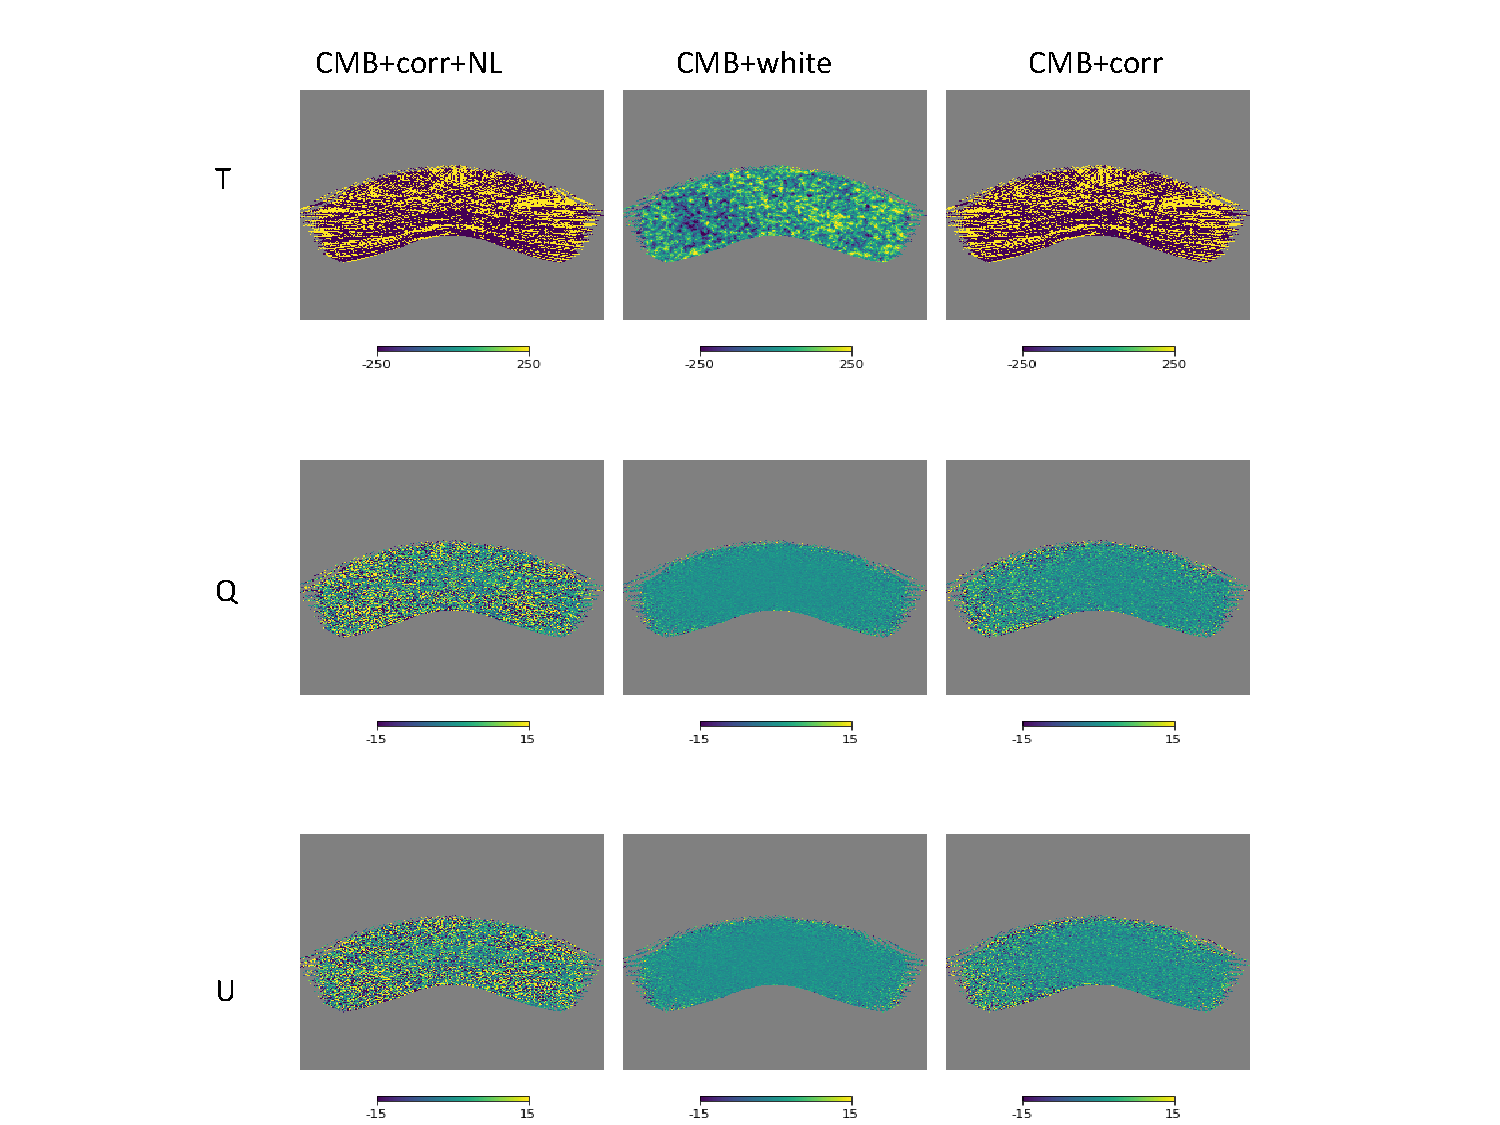
\includegraphics[width=0.85\textwidth]{figures/040218_s4cmb_corr_NL.pdf}
\caption{Pure T->P leakage maps generated with s4cmb for an example instrument and experiment. The middle column is pure CMB+white noise (minimal leakage), the right column is CMB+white+correlated noise, and the left is the same as the right but observed through the nonlinearity equation. Random draws of $g_1$ and $\tau_1$ were performed for each detector in the focal plane.}
\end{figure}

\paragraph{Uncertainty/Range:}
Current results from \cite{PB1_WHWP} quote rough estimates of $g_1 \sim$ 0.8 \%/K and $\tau_1 \sim$ 0.1 ms/K, where we assume $d(t)$ have been calibrated to CMB temperature using a conversion factor. Data for Advanced ACTPol detectors in the field with no sky loading show XX\% ratio of second-harmonic to first-harmonic amplitude.

\paragraph{Parameterization:}
We currently plan to use the simpler equation to determine what acceptable limits on $g_1$ and $\tau_1$ are demanded by science goals. When summarized in terms of TES design parameters, we can then feed these requirements back to the detector design group.

\section{Atmospheric Effects}

\section{Papers on systematics}

\input{tex/papers.tex}


 

%----------------------------------------------------------------------------------------
%	BIBLIOGRAPHY
%----------------------------------------------------------------------------------------

\renewcommand{\refname}{\spacedlowsmallcaps{References}} % For modifying the bibliography heading
\bibliographystyle{unsrt}
\bibliography{syst.bib} % The file containing the bibliography

%----------------------------------------------------------------------------------------

\end{document}
